\section*{Introduction}
Dans le chapitre précédent, nous avons défini les besoins liés à notre solution et réparti les différentes tâches du projet afin que les phases de travail soient correctement planifiées.
\newline Au cours de ce chapitre, nous présenterons les fonctionnalités liées  à la gestion des utilisateurs, à l'authentification et au contrôle d'accès basé sur les rôles (RBAC), retenues dans le cadre du premier sprint de notre projet.

% ─────────────────────────────────────────────────────────────────────────────
% SECTION 1 : BACKLOG DU SPRINT 1
% ─────────────────────────────────────────────────────────────────────────────
\section{Sprint Planning Meeting }
La planification du sprint est essentielle à la réussite de notre solution, au bout de laquelle on clarifie les différentes fonctionnalités à implémenter lors du sprint à venir. Cette partie est efficace afin de préparer des objectifs clairs.
L'objectif de ce sprint est de mettre en place les fondations fonctionnelles et
sécuritaires de la solution, en implémentant les mécanismes d'authentification et
de sécurisation des accès ainsi que les fonctionnalités de gestion des utilisateurs
et de leurs profils. Il s'agit également d'assurer un contrôle efficace des accès
et des permissions en introduisant l'administration du système à travers la gestion
des comptes utilisateurs, des rôles et des permissions (RBAC).
\subsection{Backlog du premier sprint}
\label{sec:backlog_sprint1}

Voici l'ensemble des fonctionnalités issues du Product Backlog, qui seront réalisées dans le cadre de ce sprint.
\newline
\textbf{1 : Effort faible, 2 : Effort moyen, 3 : Effort élevé}
\rowcolors{0}{}{}
\arrayrulecolor{black}
\renewcommand{\arraystretch}{1.3}
\small

\begin{longtable}{|C{1cm}|m{6.5cm}|m{7cm}|C{1cm}|}
\hline
\textbf{ID US} & \textbf{User Story} & \textbf{Description technique} & \textbf{Effort} \\
\hline
\endfirsthead

    \hline

\endhead

\hline
\endfoot

\hline
\endlastfoot

% Epic 1: Authentification et Sécurité
\multicolumn{4}{|l|}{\cellcolor{blue!20}\textbf{Epic 1 - Authentification et Sécurité}} \\
\hline

US01 & En tant qu'\textbf{utilisateur}, je souhaite m'authentifier avec email et mot de passe afin d'accéder à mes informations de manière sécurisée. & 
\vspace{2mm}
\begin{itemize}[nosep, left=0pt, label={$\bullet$}]
\item Développer l'endpoint \texttt{POST /api/auth/login}
\item Mettre en place la gestion de session via \textbf{JWT}
    (access token 15 min, refresh token 7 jours stocké en base)
\item Réaliser l'interface connexion login
\item Consommer l'API d'authentification
\item Gérer les tentatives échouées (3 essais) avec verrouillage temporaire
\end{itemize} & 2 \\
\hline

US02 & En tant qu'\textbf{utilisateur}, je souhaite réinitialiser mon mot de passe afin de retrouver l'accès à mon compte. & 
\vspace{2mm}
\begin{itemize}[nosep, left=0pt, label={$\bullet$}]
\item Développer les endpoints
    \texttt{POST /api/auth/mot-de-passe-oublie} et
    \texttt{POST /api/auth/reinitialiser-mot-de-passe}
  \item Créer les formulaires « mot de passe oublié » et
    de réinitialisation côté Next.js
  \item Générer un token sécurisé (bcrypt) avec expiration
    de \textbf{1 heure}, stocké dans
    \texttt{TokenReinitialisationMotDePasse}
  \item Invalider les anciens tokens non utilisés à chaque
    nouvelle demande
  \item Configurer l'envoi d'un e-mail de réinitialisation
    et d'un e-mail de confirmation via \textbf{Nodemailer}
\end{itemize} & 2 \\
\hline

US03 & En tant qu'\textbf{utilisateur}, je souhaite m'authentifier via Google ou GitHub afin de me connecter rapidement sans créer de compte. & 
\vspace{2mm}
\begin{itemize}[nosep, left=0pt, label={$\bullet$}]
\item Intégrer les stratégies OAuth2 via
    \texttt{passport-google-oauth20} et \texttt{passport-github2}
    dans NestJS (\texttt{@nestjs/passport})
\item Implémenter les routes \texttt{GET /api/auth/google},\texttt{GET /api/auth/github} et leurs callbacks
  \item Si l'utilisateur existe en base et est actif :
    générer les tokens JWT et rediriger vers le frontend
    avec \texttt{?oauth=success}
\item Vérifier l'existence de l'utilisateur en base de données et une demande d'inscription OAuth est envoyée à l'admin
\item Implémenter les routes /auth/google, /auth/github et leurs callbacks, avec génération d'un JWT
\item Implémenter les boutons OAuth sur la page de login
\end{itemize} & 3 \\
\hline

US04 & En tant qu'\textbf{utilisateur}, je souhaite me déconnecter de la plateforme afin de sécuriser ma session. & 
\vspace{2mm}
\begin{itemize}[nosep, left=0pt, label={$\bullet$}]
\item Développer l'endpoint POST /auth/logout avec révocation du refresh token en base
\item Supprimer \texttt{accessToken}, \texttt{refreshToken}
    et \texttt{user} du \texttt{localStorage}
\item Vider le cache React Query (\texttt{queryClient.clear()})
\item Réaliser le bouton de déconnexion 
\end{itemize} & 1 \\
\hline

US05 & En tant qu'\textbf{utilisateur}, je souhaite que mon compte soit protégé contre les tentatives de connexion malveillantes afin de garantir la sécurité de mes données. & 
\vspace{2mm}
\begin{itemize}[nosep, left=0pt, label={$\bullet$}]
  \item Implémenter le compteur de tentatives échouées
    (\texttt{tentativesConnexionEchouees}) en base de données
  \item Verrouiller le compte après \textbf{3 tentatives échouées}
    pendant \textbf{1 minute} via le champ
    \texttt{compteVerrouilleJusquA}
  \item Réinitialiser le compteur à 0 après une connexion réussie
  \item Appliquer le rate limiting global via
    \texttt{@nestjs/throttler} sur les endpoints publics
\end{itemize} & 2 \\
\hline

% Epic 2: Gestion des utilisateurs
\multicolumn{4}{|l|}{\cellcolor{blue!20}\textbf{Epic 2 - Gestion des utilisateurs}} \\
\hline

US06 & En tant qu'\textbf{utilisateur}, je souhaite gérer mon profil afin que mes informations soient toujours à jour. & 
\vspace{2mm}
\begin{itemize}[nosep, left=0pt, label={$\bullet$}]
\item Développer les endpoints \texttt{GET /api/profil} et \texttt{PUT /api/profil}
\item Implémenter l'upload de la photo de profil \texttt{POST /api/profil/upload-photo}
\item Développer le changement de mot de passe via
    \texttt{POST /api/profil/change-password}
    avec vérification de l'ancien mot de passe (bcrypt)
\item Gérer les e-mails secondaires :
    \texttt{GET/POST/DELETE /api/profil/emails} et
    \texttt{PATCH /api/profil/emails/principal}
\item Réaliser l'interface profil côté Next.js  avec formulaire prérempli
\end{itemize} & 2 \\
\hline

US07 & En tant qu'\textbf{administrateur}, je souhaite créer des utilisateurs afin de gérer les accès au système. & 
\vspace{2mm}
\begin{itemize}[nosep, left=0pt, label={$\bullet$}]
\item Développer l'endpoint \texttt{POST /api/users}
\item Générer automatiquement un mot de passe temporaire haché via \textbf{bcrypt} (facteur 10)
\item Générer un token de réinitialisation (1 heure) et construire le lien de réinitialisation
\item Créer automatiquement le \texttt{ProfilEmploye}
    avec matricule \texttt{EMP-\{id\}} si le rôle n'est pas CLIENT
\item Valider les données d'entrée via \textbf{class-validator}
  \item Envoyer un e-mail de bienvenue via \textbf{Nodemailer}
    contenant le mot de passe temporaire et le lien de
    réinitialisation
  \item Réaliser le formulaire d'ajout côté Next.js
\end{itemize} & 3 \\
\hline

US08 & En tant qu'\textbf{administrateur}, je souhaite modifier les informations d'un utilisateur afin de maintenir des données à jour. & 
\vspace{2mm}
\begin{itemize}[nosep, left=0pt, label={$\bullet$}]
\item Développer l'endpoint \texttt{PUT /api/users/:id}
\item Sécuriser l'accès à l'endpoint pour les administrateurs uniquement
\item Valider les données via \textbf{class-validator}
\item Réaliser le formulaire de modification côté Next.js
\end{itemize} & 2 \\
\hline

US09 & En tant qu'\textbf{administrateur}, je souhaite activer et désactiver un compte utilisateur afin de contrôler l'accès au système. & 
\vspace{2mm}
\begin{itemize}[nosep, left=0pt, label={$\bullet$}]
\item Développer les endpoints \texttt{PATCH /api/users/:id/desactiver} et \texttt{PATCH /api/users/:id/reactiver}
\item Implémenter les vérifications de réassignation des tickets et des demandes en cas de désactivation
\item Envoyer des notifications pour informer l'utilisateur de l'activation ou désactivation de son compte
\item Réaliser les boutons d'action avec appels des API
\end{itemize} & 3 \\
\hline

US10 & En tant qu'\textbf{administrateur}, je souhaite consulter la liste des utilisateurs afin de visualiser et gérer efficacement les comptes. & 
\vspace{2mm}
\begin{itemize}[nosep, left=0pt, label={$\bullet$}]
\item Développer l'endpoint \texttt{GET /api/users}
\item Réaliser l'interface d'administration avec vue grille
    et vue liste, filtres par statut et par rôle,
    barre de recherche dynamique

\end{itemize} & 1 \\
\hline

US11 & En tant qu'\textbf{utilisateur}, je souhaite consulter l'historique de mes activités afin de suivre mes actions dans le système. & 
\vspace{2mm}
\begin{itemize}[nosep, left=0pt, label={$\bullet$}]
\item Développer l'endpoint \texttt{GET /api/users/:id/activities} pour récupérer l'historique
\item Implémenter la logique de filtrage dans le backend en utilisant l'opérateur contains
\item Implémenter une barre de recherche dynamique
\item Réaliser l'interface timeline avec filtres par date et type d'action
\end{itemize} & 2 \\
\hline

% Epic 3: Gestion des rôles et permissions
\multicolumn{4}{|l|}{\cellcolor{blue!20}\textbf{Epic 3 - Gestion des rôles et permissions}} \\
\hline

US12 & En tant qu'\textbf{administrateur}, je souhaite gérer des rôles afin de structurer les accès au système. & 
\vspace{2mm}
\begin{itemize}[nosep, left=0pt, label={$\bullet$}]
\item Développer les endpoints CRUD pour la gestion complète des rôles
\item Implémenter le PermissionsGuard et le décorateur @Permissions pour sécuriser les routes du backend 
\item Réaliser l'interface de gestion sous forme de matrice
\end{itemize} & 3 \\
\hline

US13 & En tant qu'\textbf{administrateur}, je souhaite attribuer des permissions granulaires aux rôles afin de contrôler précisément les accès. & 
\vspace{2mm}
\begin{itemize}[nosep, left=0pt, label={$\bullet$}]
\item Développer l’endpoint PATCH /roles-permissions/roles/:id/sync pour synchroniser dynamiquement les associations entre un rôle et ses permissions. 
\item Implémenter la logique de mise à jour atomique                                                                                                                                                                                                                       
\item Développer l'interface interactive de type "Matrice de contrôle d'accès" 

\end{itemize} & 2 \\
\hline
US14 & En tant qu'\textbf{administrateur}, je souhaite consulter la matrice rôles-permissions afin de visualiser rapidement les droits de chaque rôle. & 
\vspace{2mm}
\begin{itemize}[nosep, left=0pt, label={$\bullet$}]
\item Développer l’endpoint GET /roles-permissions/matrix ) pour récupérer les données 
\item Implémenter la logique de structuration des données au format JSON                
\item Réaliser l’interface de visualisation de type "Heatmap" ou "Tableau de bord"

\end{itemize} & 3 \\
\hline

% Epic 4: Demandes d'inscription OAuth
\multicolumn{4}{|l|}{\cellcolor{blue!20}\textbf{Epic 4 - Demandes d'inscription OAuth}} \\
\hline

US15 & En tant qu'\textbf{utilisateur externe}, je souhaite demander l'accès via OAuth afin de m'inscrire facilement. & 
\vspace{2mm}
\begin{itemize}[nosep, left=0pt, label={$\bullet$}]
\item Développer l'endpoint POST /auth/oauth/request pour créer une demande
\item Enregistrer la demande en base avec statut EN\_ATTENTE
\item Implémenter l'envoi de notification à l'administrateur via email et in-app
\item Réaliser l'interface de demande d'accès
\end{itemize} & 3 \\
\hline

US16 & En tant qu'\textbf{administrateur}, je souhaite valider ou rejeter les demandes d'inscription OAuth afin de contrôler les accès. & 
\vspace{2mm}
\begin{itemize}[nosep, left=0pt, label={$\bullet$}]
\item Développer les endpoints PATCH /auth/oauth/requests/:id/approve et /reject
\item Implémenter la création automatique du compte utilisateur lors de l'approbation
\item Configurer l'envoi d'emails de confirmation ou rejet via Nodemailer
\item Réaliser l'interface de gestion des demandes avec actions d'approbation/rejet
\end{itemize} & 3 \\
\hline
% Epic 4: Demandes d'inscription OAuth


\end{longtable}



% ─────────────────────────────────────────────────────────────────────────────
% SECTION 2 : ANALYSE
% ─────────────────────────────────────────────────────────────────────────────

\section{Analyse}
Dans le processus de développement, l'analyse joue un rôle important ; elle permet d'identifier les exigences du système et de traduire les besoins exprimés en spécifications claires et cohérentes.
C'est pour cela que nous allons présenter les diagrammes ainsi que les tableaux descriptifs des cas d'utilisation
\label{sec:analyse_sprint1}

\subsection{Diagramme des cas d'utilisation du premier sprint}

La figure ci-dessous présente le diagramme de cas d'utilisation du premier sprint : 
\begin{figure}[htbp]
        \centering
        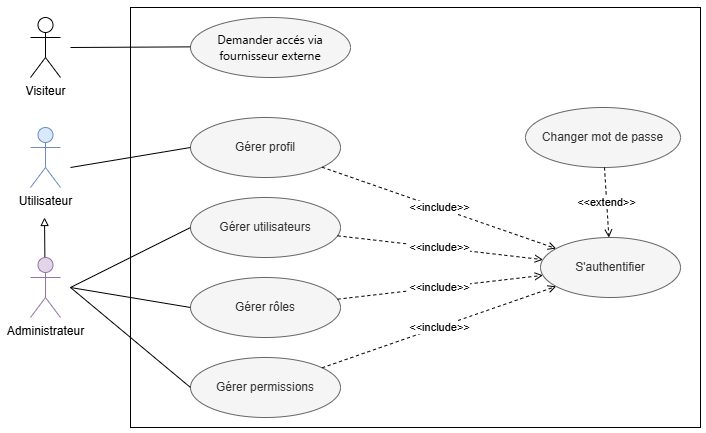
\includegraphics[width=0.75\textwidth,height=0.65\textheight,keepaspectratio]{Images/Diagramme_cas_utilisation_sprint1.png}
        \caption{Diagramme des cas d'utilisation du premier sprint}
        \label{fig:use_case_sprint1}
\end{figure}

Nous allons accompagner les cas d'utilisation d'un texte descriptif pour expliquer le scénario de chaque cas ainsi que ses exceptions.

\subsection{Description textuelle de cas d'utilisation «S'authentifier»}
La figure ci-dessous présente la description textuelle de cas d'utilisation «S'authentifier» :

\footnotesize
\renewcommand{\arraystretch}{0.95}
\begin{longtable}{|P{3.5cm}|P{10.5cm}|}
\caption{Description textuelle du cas d'utilisation « S'authentifier »} \\
\hline
\endfirsthead
\hline
\endhead
\hline
\endfoot
\hline
\endlastfoot
\textbf{Nom du cas d'utilisation} & S'authentifier \\
\hline
\textbf{Acteurs} & Utilisateur \\
\hline
\textbf{Préconditions} & L'utilisateur dispose déjà d'un compte actif \\
\hline
\textbf{Postconditions} & L'utilisateur est authentifié et reçoit un jeton d'accès ainsi qu'un jeton de rafraîchissement \\
\hline
\textbf{Scénario principal} &
\begin{minipage}[t]{\linewidth}\raggedright
\begin{enumerate}[label=\arabic*., nosep,leftmargin=0.6cm,topsep=0pt,itemsep=1pt]
\item Le système affiche le formulaire de connexion.
\item L'utilisateur saisit son adresse e-mail et son mot de passe.
\item L'utilisateur valide la connexion.
\item Le système vérifie l'existence du compte.
\item Le système vérifie la validité du mot de passe.
\item Le système vérifie que le compte est actif.
\item Le système détermine le profil de l'utilisateur et récupère ses rôles et permissions.
\item Le système met à jour la date de dernière connexion.
\item Le système génère un jeton d'accès et un jeton de rafraîchissement.
\item Le système renvoie les informations de l'utilisateur connecté.
\item Le système redirige l'utilisateur vers la page d'accueil ou le tableau de bord.
\end{enumerate}
\end{minipage} \\
\hline
\textbf{Scénarios alternatifs} &
\begin{itemize}[nosep,leftmargin=0.6cm,topsep=0pt,itemsep=1pt, label=$\bullet$]
\item L'utilisateur s'authentifie via Google.
\item L'utilisateur s'authentifie via GitHub.
\end{itemize} \\
\hline
\textbf{Scénarios d'exception} &
\begin{itemize}[nosep,leftmargin=0.6cm,topsep=0pt,itemsep=1pt, label=$\bullet$]
\item L'utilisateur saisit un identifiant inexistant.
\item L'utilisateur saisit un mot de passe incorrect.
\item Le compte de l'utilisateur est désactivé.
\item Le formulaire contient des champs obligatoires vides ou invalides.
\item Le compte est temporairement verrouillé après \textbf{3 tentatives échouées} consécutives (durée : 1 minute).
\end{itemize} \\
\hline
\end{longtable}
\normalsize
\vspace{-0.3cm}


\subsection{Description textuelle de cas d'utilisation « Changer mot de passe »}
La figure ci-dessous présente la description textuelle du cas d'utilisation « Changer le mot de passe » :

\footnotesize
\renewcommand{\arraystretch}{0.95}
\begin{longtable}{|P{3.5cm}|P{10.5cm}|}
\caption{Description textuelle de cas d'utilisation « Changer mot de passe »} \\
\hline
\endfirsthead
\hline
\endhead
\hline
\endfoot
\hline
\endlastfoot
\textbf{Nom du cas d'utilisation} & Changer mot de passe \\
\hline
\textbf{Acteurs} & Utilisateurs \\
\hline
\textbf{Préconditions} & L'utilisateur possède déjà un compte \\
\hline
\textbf{Postconditions} & Le mot de passe est réinitialisé \\
\hline
\textbf{Scénario principal} &
\begin{minipage}[t]{\linewidth}\raggedright
\begin{enumerate}[label=\arabic*., nosep,leftmargin=0.6cm,topsep=0pt,itemsep=1pt]
\item Le système affiche un formulaire de changement de mot de passe.
\item L'utilisateur saisit son e-mail.
\item L'utilisateur clique sur le bouton « Réinitialiser le mot de passe ».
\item Le système vérifie l'existence de l'email.
\item Le système envoie un e-mail à l'utilisateur.
\item L'utilisateur clique sur le lien reçu par e-mail.
\item Le système affiche le formulaire de réinitialisation de mot de passe.
\item L'utilisateur saisit son nouveau mot de passe deux fois pour confirmation.
\item Le système valide et enregistre le nouveau mot de passe.
\item Le système envoie un e-mail de confirmation à l'utilisateur.
\end{enumerate}
\end{minipage} \\
\hline
\textbf{Scénarios d'exception} &
\begin{itemize}[nosep,leftmargin=0.6cm,topsep=0pt,itemsep=1pt, label=$\bullet$]
\item L'utilisateur saisit un e-mail qui ne correspond à aucun compte existant.
\item L'utilisateur a rempli un champ invalide, ou a laissé un champ vide.
\item Le lien de réinitialisation est expiré.
\item L'utilisateur ne confirme pas correctement le mot de passe.
\end{itemize} \\
\hline
\end{longtable}
\normalsize
\vspace{-0.3cm}

\subsection{Analyse de la fonctionnalité « Demander accès via fournisseur externe »}
Dans cette partie, nous allons présenter les cas d'utilisation raffinés relatifs à la demande d'accès via fournisseur externe afin de comprendre les différentes étapes du processus d'inscription et d'authentification.

\subsubsection{Raffinement de cas d'utilisation « Demander accés via fournisseur externe »}
Au cours de cette partie, nous allons analyser les sous-cas d'utilisation pour le processus d'authentification OAuth :

\begin{figure}[htbp]
        \centering
        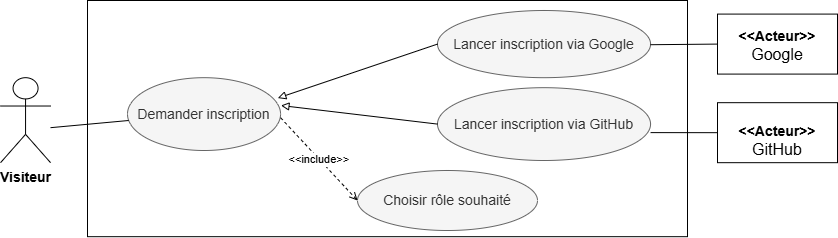
\includegraphics[width=0.75\textwidth,height=0.65\textheight,keepaspectratio]{Images/demande insc.png}
        \caption{Raffinement de cas d'utilisation « Demander accés via fournisseur externe »}
        \label{fig:oauth_refinement}
\end{figure}

\subsubsection{Description textuelle de cas d'utilisation « Soumettre demande d'inscription »}

\footnotesize
\renewcommand{\arraystretch}{0.95}
{\sloppy
\begin{longtable}{|P{3.5cm}|P{10.5cm}|}
\caption{Description textuelle « Soumettre demande d'inscription »} \\
\hline
\endfirsthead
\hline
\endhead
\hline
\endfoot
\hline
\endlastfoot
\textbf{Nom du cas d'utilisation} & Soumettre demande d'inscription \\
\hline
\textbf{Acteurs} & Visiteur \\
\hline
\textbf{Préconditions} & Le visiteur n'a pas de compte actif dans le système et a accès à la page d'authentification \\
\hline
\textbf{Postconditions} &
\begin{minipage}[t]{\linewidth}\raggedright\hyphenpenalty=1000
La demande d'inscription est créée, enregistrée avec le statut \textbf{EN\_ATTENTE}, et les administrateurs sont notifiés
\end{minipage} \\\hline
\textbf{Scénario principal} &
\begin{minipage}[t]{\linewidth}\raggedright
\begin{enumerate}[label=\arabic*., leftmargin=0.6cm, nosep, itemsep=1pt]
\item Le visiteur accède à la page de connexion / inscription.
\item Le visiteur sélectionne le rôle souhaité : Client, Développeur ou Chef de projet.
\item Le visiteur clique sur « Se connecter avec Google » ou « Se connecter avec GitHub ».
\item Le système redirige le visiteur vers le fournisseur OAuth sélectionné.
\item Le visiteur s'authentifie et autorise l'application à accéder à ses informations de base.
\item Le fournisseur OAuth redirige le visiteur vers l'application avec un code d'autorisation.
\item Le système récupère les informations du profil OAuth et vérifie s'il existe déjà un compte actif associé.
\item Si aucun compte actif n'existe, le système crée une demande d'inscription avec le statut \textit{EN ATTENTE}.
\item Le système envoie une \textbf{notification interne} et un \textbf{e-mail} à chaque administrateur actif pour l'informer de la nouvelle demande d'inscription.
\item Le système envoie un \textbf{e-mail de confirmation au visiteur} indiquant que sa demande a bien été reçue et est en cours d'examen.
\item Le système affiche un message d'attente à l'écran.
\end{enumerate}
\end{minipage} \\
\hline
\textbf{Scénarios alternatifs} &
\begin{itemize}[nosep,leftmargin=0.6cm,topsep=0pt,itemsep=1pt, label=$\bullet$]
\item Compte actif déjà existant : le système connecte directement l'utilisateur sans créer de nouvelle demande.
\item Demande déjà soumise pour le même e-mail et le même fournisseur : le système conserve la demande existante et affiche un message d'information, sans créer de doublon.
\item Annulation de l'autorisation OAuth : le visiteur est redirigé vers la page d'authentification sans création de demande.
\end{itemize} \\
\hline
\textbf{Scénarios d'exception} &
\begin{itemize}[nosep,leftmargin=0.6cm,topsep=0pt,itemsep=1pt, label=$\bullet$]
\item Le fournisseur OAuth ne fournit pas l'adresse e-mail : le système affiche un message d'erreur et interrompt le traitement.
\item Le fournisseur OAuth est indisponible : le système affiche un message d'erreur technique.
\item Le visiteur refuse l'accès aux données OAuth : le système annule le flux et revient à l'écran d'authentification.
\end{itemize} \\
\hline
\end{longtable}
}
\normalsize
\vspace{-0.3cm}

\subsubsection{Description textuelle de cas d'utilisation « Valider demande »}

\footnotesize
\renewcommand{\arraystretch}{0.95}
\begin{longtable}{|P{3.5cm}|P{10.5cm}|}
\caption{Description textuelle « Valider demande »} \\
\hline
\endfirsthead
\hline
\endhead
\hline
\endfoot
\hline
\endlastfoot
\textbf{Nom du cas d'utilisation} & Valider demande \\
\hline
\textbf{Acteurs} & Administrateur \\
\hline
\textbf{Préconditions} & L'administrateur est authentifié et possède la permission de traiter les demandes d'inscription \\
\hline
\textbf{Postconditions} & Le compte utilisateur est créé et activé, la demande est marquée \textit{APPROUVEE}, et l'utilisateur est notifié \\
\hline
\textbf{Scénario principal} &
\begin{minipage}[t]{\linewidth}\raggedright
\begin{enumerate}[label=\arabic*., leftmargin=0.6cm, nosep, itemsep=1pt]
\item L'administrateur accède au module de gestion des demandes d'inscription.
\item Le système affiche la liste des demandes en attente.
\item L'administrateur sélectionne une demande à traiter.
\item Le système affiche les informations du demandeur récupérées via OAuth.
\item L'administrateur clique sur « Approuver ».
\item Le système crée le compte utilisateur à partir des informations de la demande.
\item Le système attribue le rôle correspondant à l'utilisateur.
\item Le système marque la demande comme \textit{APPROUVEE}.
\item Le système envoie un e-mail de confirmation à l'utilisateur.
\item Le système affiche un message de succès à l'administrateur.
\end{enumerate}
\end{minipage} \\
\hline
\textbf{Scénarios alternatifs} &
\begin{itemize}[nosep,leftmargin=0.6cm,topsep=0pt,itemsep=1pt, label=$\bullet$]
\item L'administrateur clique sur « Refuser » : le système ouvre une boîte de dialogue pour saisir un motif de refus puis traite la demande comme rejetée.
\item Un compte avec le même e-mail existe déjà : le système signale le conflit et empêche la création d'un doublon.
\item La demande a déjà été traitée : le système affiche un message d'information et empêche une nouvelle validation.
\end{itemize} \\
\hline
\textbf{Scénarios d'exception} &
\begin{itemize}[nosep,leftmargin=0.6cm,topsep=0pt,itemsep=1pt, label=$\bullet$]
\item Erreur lors de la création du compte : le système annule l'opération et affiche un message d'erreur.
\item Erreur lors de l'envoi de l'e-mail : le compte peut être créé, mais le système journalise l'incident et affiche un avertissement.
\item Données de finalisation incomplètes : le système refuse la validation et demande de compléter les champs obligatoires.
\end{itemize} \\
\hline
\end{longtable}
\normalsize
\vspace{-0.3cm}

\subsection{Analyse de la fonctionnalité « Gérer utilisateurs »}
Dans cette partie, nous allons présenter les cas d'utilisation relatifs à la gestion des utilisateurs afin de comprendre les principales fonctionnalités du système, ce qui permet d'avoir une vue globale des interactions.
\subsubsection{Raffinement de cas d'utilisation « Gérer utilisateurs »}
Au cours de cette partie, nous allons analyser chaque cas d'utilisation raffiné pour le cas de gestion des utilisateurs :    

\begin{figure}[htbp]
        \centering
        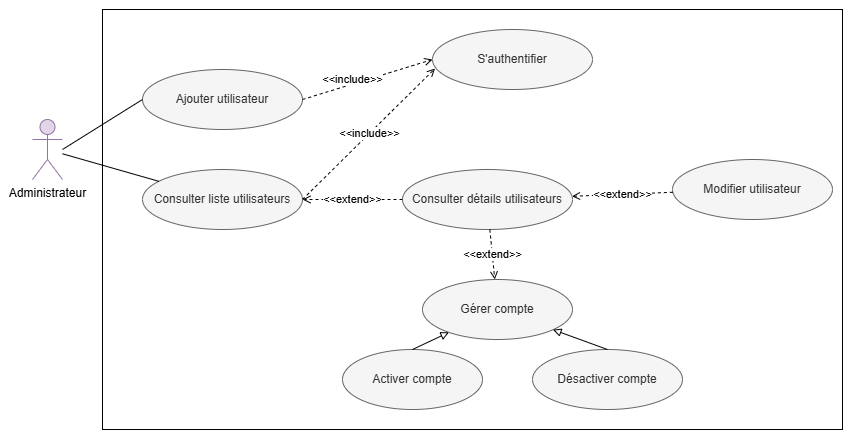
\includegraphics[width=0.8\textwidth,keepaspectratio]{Images/Gérer utilisateur.drawio.png}
        \caption{Diagramme des cas d'utilisation « Gérer utilisateurs »}
        \label{fig:gerer_utilisateurs}
\end{figure}

% \subsubsection{Description textuelle de cas d'utilisation « Consulter liste utilisateurs »}
% 
% \footnotesize
% \renewcommand{\arraystretch}{0.95}
% \begin{longtable}{|P{3.5cm}|P{10.5cm}|}
% \caption{Description textuelle « Consulter liste utilisateurs »} \\
% \hline
% \endfirsthead
% \hline
% \endhead
% \hline
% \endfoot
% \hline
% \endlastfoot
% \textbf{Nom du cas d'utilisation} & Consulter liste utilisateurs \\
% \hline
% \textbf{Acteurs} & Administrateur \\
% \hline
% \textbf{Préconditions} & L'utilisateur est authentifié\newline L'utilisateur possède la permission de consulter les utilisateurs \\
% \hline
% \textbf{Postconditions} & Liste des utilisateurs affichée \\
% \hline
% \textbf{Scénario principal} &
% \begin{minipage}[t]{\linewidth}
% \begin{enumerate}[label=\arabic*., leftmargin=0.6cm, nosep, itemsep=1pt]
%     \item L'administrateur accède à la section "Utilisateurs".
%     \item Le système affiche les utilisateurs sous forme de grille (par défaut) ou de liste selon le choix de l'utilisateur.
%     \item L'administrateur recherche un utilisateur en saisissant des informations clés dans la barre de recherche ou par des boutons de filtre (par statut, par rôle).
%     \item Le système filtre la liste.
% \end{enumerate}
% % \end{minipage} \\
% \hline
% \textbf{Scénarios alternatifs} & L'administrateur clique sur le bouton « Exporter ». \\
% \hline
% \end{longtable}
% \normalsize
% \vspace{-0.3cm}

\subsubsection{Description textuelle de cas d'utilisation « Ajouter utilisateur »}

\footnotesize
\renewcommand{\arraystretch}{0.95}
\begin{longtable}{|P{3.5cm}|P{10.5cm}|}
\caption{Description textuelle « Ajouter utilisateur »} \\
\hline
\endfirsthead
\hline
\endhead
\hline
\endfoot
\hline
\endlastfoot
\textbf{Nom du cas d'utilisation} & Ajouter utilisateur \\
\hline
\textbf{Acteurs} & Administrateur \\
\hline
\textbf{Préconditions} & L'utilisateur est authentifié\newline L'utilisateur possède la permission de créer des utilisateurs\newline Liste des utilisateurs affichée \\
\hline
\textbf{Postconditions} & Utilisateur est ajouté \\
\hline
\textbf{Scénario principal} &
\begin{minipage}[t]{\linewidth}\raggedright
\begin{enumerate}[label=\arabic*., leftmargin=0.6cm, nosep, itemsep=1pt]
    \item L'administrateur clique sur le bouton "Nouvel Utilisateur".
    \item Le système affiche le formulaire d'ajout.
    \item L'administrateur remplit le formulaire.
    \item L'administrateur valide le formulaire en cliquant sur (Créer le compte).
    \item Le système affiche le message de succès.
\end{enumerate}
\end{minipage} \\
\hline
\textbf{Scénarios d'exception} &
\begin{itemize}[nosep,leftmargin=0.6cm,topsep=0pt,itemsep=1pt, label=$\bullet$]
\item L'administrateur a rempli un champ invalide, ou a laissé un champ vide.
\item L'administrateur saisit un e-mail déjà utilisé dans un autre compte.
\item L'administrateur tente de fermer la fenêtre alors qu'il a commencé à saisir des données.
\end{itemize} \\
\hline
\textbf{Scénarios alternatifs} & Le système génère un mot de passe temporaire. \\
\hline
\end{longtable}
\normalsize
\vspace{-0.3cm}

\subsubsection{Description textuelle de cas d'utilisation « Désactiver un utilisateur »}

\footnotesize
\renewcommand{\arraystretch}{0.95}
\begin{longtable}{|P{3.5cm}|P{10.5cm}|}
\caption{Description textuelle « Désactiver un utilisateur »} \\
\hline
\endfirsthead
\hline
\endhead
\hline
\endfoot
\hline
\endlastfoot
\textbf{Nom du cas d'utilisation} & Désactiver un utilisateur \\
\hline
\textbf{Acteurs} & Administrateur \\
\hline
\textbf{Préconditions} & L'utilisateur est authentifié\newline L'utilisateur possède la permission de désactiver les utilisateurs\newline Liste des utilisateurs affichée\newline L'utilisateur à désactiver doit être actuellement Actif \\
\hline
\textbf{Postconditions} & Le compte est désactivé \\
\hline
\textbf{Scénario principal} &
\begin{minipage}[t]{\linewidth}\raggedright
\begin{enumerate}[label=\arabic*., leftmargin=0.6cm, nosep, itemsep=1pt]
    \item L'administrateur choisit un compte dans la liste.
    \item L'administrateur clique sur l'action (Désactiver).
    \item Le système vérifie si l'utilisateur possède des tickets actifs ou des demandes en attente.
    \item Le système affiche une boîte de dialogue de confirmation.
    \item L'administrateur confirme l'action.
    \item Le système met à jour le statut de l'utilisateur.
    \item Le système envoie un e-mail automatique à l'utilisateur pour l'informer de la suspension de son compte.
\end{enumerate}
\end{minipage} \\
\hline
\textbf{Scénarios alternatifs} & L'administrateur réassigne les tickets ou les demandes. \\
\hline
\textbf{Scénarios d'exception} &
\begin{itemize}[nosep,leftmargin=0.6cm,topsep=0pt,itemsep=1pt, label=$\bullet$]
\item L'utilisateur tente de désactiver un utilisateur qui possède des tickets actifs ou des demandes en attente.
\end{itemize} \\
\hline
\end{longtable}
\normalsize
\vspace{-0.3cm}

\subsubsection{Description textuelle de cas d'utilisation « Modifier Profil »}

\footnotesize
\renewcommand{\arraystretch}{0.95}
\begin{longtable}{|P{3.5cm}|P{10.5cm}|}
\caption{Description textuelle « Modifier le Profil »} \\
\hline
\endfirsthead
\hline
\endhead
\hline
\endfoot
\hline
\endlastfoot
\textbf{Nom du cas d'utilisation} & Modifier le Profil \\
\hline
\textbf{Acteurs} & Administrateur, Utilisateur \\
\hline
\textbf{Préconditions} & L'utilisateur est authentifié\newline L'utilisateur possède la permission de modifier son propre profil ou celui d'autres utilisateurs (selon le rôle) \\
\hline
\textbf{Postconditions} & Le Profil est modifié \\
\hline
\textbf{Scénario principal pour Modifier le profil d'un utilisateur} &
\begin{minipage}[t]{\linewidth}
\begin{enumerate}[label=\arabic*., leftmargin=0.6cm, nosep, itemsep=1pt]
    \item L'administrateur accède au profil de l'utilisateur.
    \item L'administrateur modifie les accès en ajoutant et retirant des rôles système.
    \item L'administrateur change le statut du compte (désactiver ou activer).
    \item Le système valide chaque action.
\end{enumerate}
\end{minipage} \\
\hline
\textbf{Scénario principal pour Modifier son propre profil} &
\begin{minipage}[t]{\linewidth}
\begin{enumerate}[label=\arabic*., leftmargin=0.6cm, nosep, itemsep=1pt]
    \item L'utilisateur accède à sa page "Mon profil".
    \item L'utilisateur met à jour sa photo de profil ou ses coordonnées.
    \item L'utilisateur change son mot de passe en saisissant son ancien mot de passe pour validation.
    \item L'utilisateur ajoute ou définit un nouvel e-mail et choisit lequel serait le principal.
    \item Le système enregistre les changements.
\end{enumerate}
\end{minipage} \\
\hline
\textbf{Scénarios d'exception} &
\begin{itemize}[nosep,leftmargin=0.6cm,topsep=0pt,itemsep=1pt, label=$\bullet$]
\item L'administrateur veut retirer le dernier rôle.
\item L'utilisateur veut modifier ses propres rôles.
\end{itemize} \\
\hline
\end{longtable}
\normalsize
\vspace{-0.3cm}

\subsection{Analyse de la fonctionnalité « Gérer rôles »}
Dans cette partie, nous allons présenter les cas d'utilisation relatifs à la gestion des rôles afin
de comprendre les principales fonctionnalités du système, ce qui permet d'avoir une vue globale des
interactions.
\subsubsection{Raffinement de cas d'utilisation « Gérer rôles »}
Au cours de cette partie, nous allons analyser chaque cas d'utilisation raffiné pour le cas de gestion des rôles :

\begin{figure}[htbp]
\centering
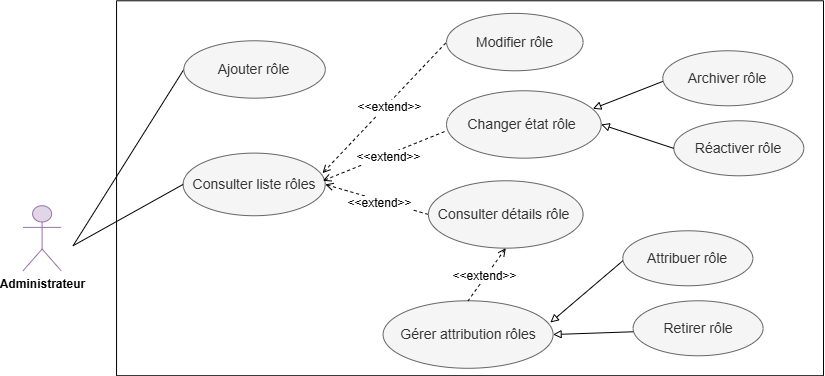
\includegraphics[width=0.8\textwidth,keepaspectratio]{Images/diag cas d'utilisation role.drawio.png}
\caption{Raffinement de cas d'utilisation « Gérer rôles »}
\label{fig:gerer_roles}
\end{figure}

\subsubsection{Description textuelle de cas d'utilisation « Archiver rôle »}

\footnotesize
\renewcommand{\arraystretch}{0.95}
\begin{longtable}{|P{3.5cm}|P{10.5cm}|}
\caption{Description textuelle « Archiver rôle »} \\
\hline
\endfirsthead
\hline
\endhead
\hline
\endfoot
\hline
\endlastfoot
\textbf{Nom du cas d'utilisation} & Archiver rôle \\
\hline
\textbf{Acteurs} & Administrateur \\
\hline
\textbf{Préconditions} & L'utilisateur est authentifié\newline L'utilisateur possède la permission d'archiver les rôles\newline Le rôle ne doit pas être assigné à des utilisateurs \\
\hline
\textbf{Postconditions} & Le rôle est archivé \\
\hline
\textbf{Scénario principal} &
\begin{minipage}[t]{\linewidth}\raggedright
\begin{enumerate}[label=\arabic*., leftmargin=0.6cm, nosep, itemsep=1pt]
\item L'administrateur sélectionne un rôle dans la liste.
\item L'administrateur clique sur l'action (Archiver).
\item Le système vérifie que le rôle n'est pas assigné à des utilisateurs.
\item Le système affiche une confirmation.
\item L'administrateur confirme l'action.
\item Le système marque le rôle comme archivé.
\item Le système affiche le message de succès.
\end{enumerate}
\end{minipage} \\
\hline
\textbf{Scénarios d'exception} & Le rôle est encore assigné à des utilisateurs. \\
\hline
\textbf{Scénarios alternatifs} & L'administrateur restaure un rôle archivé. \\
\hline
\end{longtable}
\normalsize
\vspace{-0.3cm}

\subsubsection{Description textuelle de cas d'utilisation « Attribuer rôle à utilisateur »}

\footnotesize
\renewcommand{\arraystretch}{0.95}
\needspace{10\baselineskip}
\begin{longtable}{|P{3.5cm}|P{10.5cm}|}
\caption{Description textuelle « Attribuer rôle à utilisateur »} \\
\hline
\endfirsthead
\hline
\endhead
\hline
\endfoot
\hline
\endlastfoot
\textbf{Nom du cas d'utilisation} & Attribuer rôle à utilisateur \\
\hline
\textbf{Acteurs} & Administrateur \\
\hline
\textbf{Préconditions} & L'utilisateur est authentifié\newline L'utilisateur possède la permission d'attribuer des rôles\newline Utilisateur et rôle existent \\
\hline
\textbf{Postconditions} & Le rôle est attribué à l'utilisateur \\
\hline
\textbf{Scénario principal} &
\begin{minipage}[t]{\linewidth}\raggedright
\begin{enumerate}[label=\arabic*., leftmargin=0.6cm, nosep, itemsep=1pt]
\item L'administrateur consulte le profil d'un utilisateur.
\item L'administrateur clique sur "Ajouter un rôle".
\item Le système affiche la liste des rôles disponibles.
\item L'administrateur sélectionne un rôle.
\item L'administrateur valide la sélection.
\item Le système vérifie les règles d'exclusivité métier :
  \begin{itemize}[nosep,label=$-$]
    \item Un utilisateur ayant le rôle \texttt{CLIENT} ne peut pas recevoir les rôles \texttt{CHEF\_PROJET} ou \texttt{DEVELOPPEUR}.
    \item Un utilisateur ayant le rôle \texttt{CLIENT} ne peut pas recevoir le rôle \texttt{ADMIN}.
    \item La combinaison \texttt{ADMIN} + \texttt{CHEF\_PROJET} est \textbf{autorisée}.
  \end{itemize}
\item Le système crée l'attribution.
\item Le système affiche le message de succès.
\end{enumerate}
\end{minipage} \\
\hline
\textbf{Scénarios alternatifs} & L'administrateur peut aussi attribuer le rôle depuis les détails du rôle en sélectionnant un ou plusieurs utilisateurs à qui l'attribuer. \\
\hline
\textbf{Scénarios d'exception} &
\begin{itemize}[nosep,leftmargin=0.6cm,topsep=0pt,itemsep=1pt, label=$\bullet$]
\item Le rôle est déjà attribué à cet utilisateur.
\item Violation des règles d'exclusivité des rôles.
\end{itemize} \\
\hline
\end{longtable}
\normalsize
\vspace{-0.3cm}

\subsubsection{Description textuelle de cas d'utilisation « Retirer rôle utilisateur »}

\footnotesize
\renewcommand{\arraystretch}{0.95}
\begin{longtable}{|P{3.5cm}|P{10.5cm}|}
\caption{Description textuelle « Retirer rôle utilisateur »} \\
\hline
\endfirsthead
\hline
\endhead
\hline
\endfoot
\hline
\endlastfoot
\textbf{Nom du cas d'utilisation} & Retirer rôle utilisateur \\
\hline
\textbf{Acteurs} & Administrateur \\
\hline
\textbf{Préconditions} & L'utilisateur est authentifié\newline L'utilisateur possède la permission de retirer des rôles\newline Le rôle est attribué à l'utilisateur \\
\hline
\textbf{Postconditions} & Le rôle est retiré de l'utilisateur \\
\hline
\textbf{Scénario principal} &
\begin{minipage}[t]{\linewidth}\raggedright
\begin{enumerate}[label=\arabic*., leftmargin=0.6cm, nosep, itemsep=1pt]
\item L'administrateur consulte le profil d'un utilisateur.
\item L'administrateur visualise les rôles actuels de l'utilisateur.
\item L'administrateur clique sur l'icône de suppression d'un rôle.
\item Le système affiche une confirmation.
\item L'administrateur confirme l'action.
\item Le système retire le rôle.
\item Le système affiche le message de succès.
\end{enumerate}
\end{minipage} \\
\hline
\textbf{Scénarios d'exception} &
\begin{itemize}[nosep,leftmargin=0.6cm,topsep=0pt,itemsep=1pt, label=$\bullet$]
\item L'administrateur tente de retirer le dernier rôle de l'utilisateur.
\item Le rôle n'est pas attribué à cet utilisateur.
\end{itemize} \\
\hline
\end{longtable}
\normalsize
\vspace{-0.3cm}

\subsection{Analyse de la fonctionnalité « Gérer permissions »}
Dans cette partie, nous allons présenter les cas d'utilisation relatifs à la gestion des permissions afin
de comprendre les principales fonctionnalités du système, ce qui permet d'avoir une vue globale des
interactions.
\subsubsection{Raffinement de cas d'utilisation « Gérer permissions »}
Au cours de cette partie, nous allons analyser chaque cas d'utilisation raffiné pour le cas de gestion des permissions :

\begin{figure}[htbp]
\centering
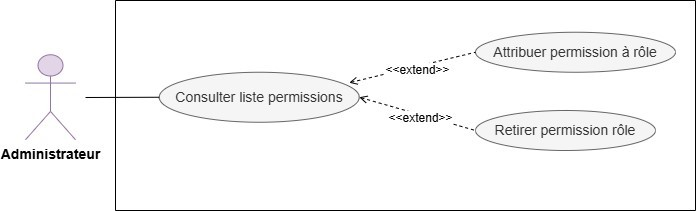
\includegraphics[width=0.8\textwidth,keepaspectratio]{Images/gerer permession.drawio.jpg}
\caption{Raffinement de cas d'utilisation « Gérer permissions »}
\label{fig:gerer_permissions}
\end{figure}

\subsubsection{Description textuelle de cas d'utilisation « Consulter liste permissions »}

\footnotesize
\renewcommand{\arraystretch}{0.95}
{\sloppy
\begin{longtable}{|P{3.5cm}|P{10.5cm}|}
\caption{Description textuelle « Consulter liste permissions »} \\
\hline
\endfirsthead
\hline
\endhead
\hline
\endfoot
\hline
\endlastfoot
\textbf{Nom du cas d'utilisation} & Consulter liste des permissions \\
\hline
\textbf{Acteurs} & Administrateur \\
\hline
\textbf{Préconditions} & L'utilisateur est authentifié\newline L'utilisateur possède la permission de consulter les permissions \\
\hline
\textbf{Postconditions} & Liste des permissions affichée \\
\hline
\textbf{Scénario principal} &
\begin{minipage}[t]{\linewidth}\raggedright
\begin{enumerate}[label=\arabic*., leftmargin=0.6cm, nosep, itemsep=1pt]
\item L'administrateur accède à la section "Permissions".
\item Le système affiche une matrice avec les rôles en horizontal et les catégories de permissions en vertical.
\item L'administrateur peut visualiser quelles permissions sont attribuées à chaque rôle (cases cochées).
\item L'administrateur peut filtrer par catégorie de permissions ou par rôle.
\end{enumerate}
\end{minipage} \\
\hline
\textbf{Scénarios alternatifs} &
\begin{itemize}[nosep,leftmargin=0.6cm,topsep=0pt,itemsep=1pt, label=$\bullet$]
\item L'administrateur sélectionne la vue "Par rôle" pour afficher une liste des rôles avec leurs permissions respectives organisées par catégorie.
\item L'administrateur clique sur le bouton « Exporter » pour télécharger la matrice des permissions.
\end{itemize} \\
\hline
\end{longtable}
}
\normalsize
\vspace{-0.3cm}

\subsubsection{Description textuelle de cas d'utilisation « Attribuer permission à rôle »}

\footnotesize
\renewcommand{\arraystretch}{0.95}
{\sloppy
\begin{longtable}{|P{3.5cm}|P{10.5cm}|}
\caption{Description textuelle « Attribuer permission à rôle »} \\
\hline
\endfirsthead
\hline
\endhead
\hline
\endfoot
\hline
\endlastfoot
\textbf{Nom du cas d'utilisation} & Attribuer permission à rôle \\
\hline
\textbf{Acteurs} & Administrateur \\
\hline
\textbf{Préconditions} & L'utilisateur est authentifié\newline L'utilisateur possède la permission d'attribuer des permissions aux rôles\newline Rôle et permission existent \\
\hline
\textbf{Postconditions} & La permission est ajoutée au rôle \\
\hline
\textbf{Scénario principal} &
\begin{minipage}[t]{\linewidth}\raggedright
\begin{enumerate}[label=\arabic*., leftmargin=0.6cm, nosep, itemsep=1pt]
\item L'administrateur consulte un rôle spécifique.
\item L'administrateur clique sur l'onglet "Permissions".
\item Le système affiche toutes les permissions organisées par catégorie avec des cases à cocher.
\item L'administrateur coche les permissions à attribuer.
\item L'administrateur clique sur "Enregistrer".
\item Le système crée les liaisons.
\item Le système affiche le message de succès.
\end{enumerate}
\end{minipage} \\
\hline
\textbf{Scénarios alternatifs} & L'administrateur utilise la matrice des permissions pour cocher les cases correspondant aux permissions à attribuer pour plusieurs rôles simultanément. \\
\hline
\textbf{Scénarios d'exception} & La permission est déjà attribuée au rôle. \\
\hline
\end{longtable}
}
\normalsize
\vspace{-0.3cm}

% ─────────────────────────────────────────────────────────────────────────────
% SECTION 3 : CONCEPTION
% ─────────────────────────────────────────────────────────────────────────────

\section{Diagramme de classes de premiére sprint}

\begin{figure}[htbp]
        \centering
        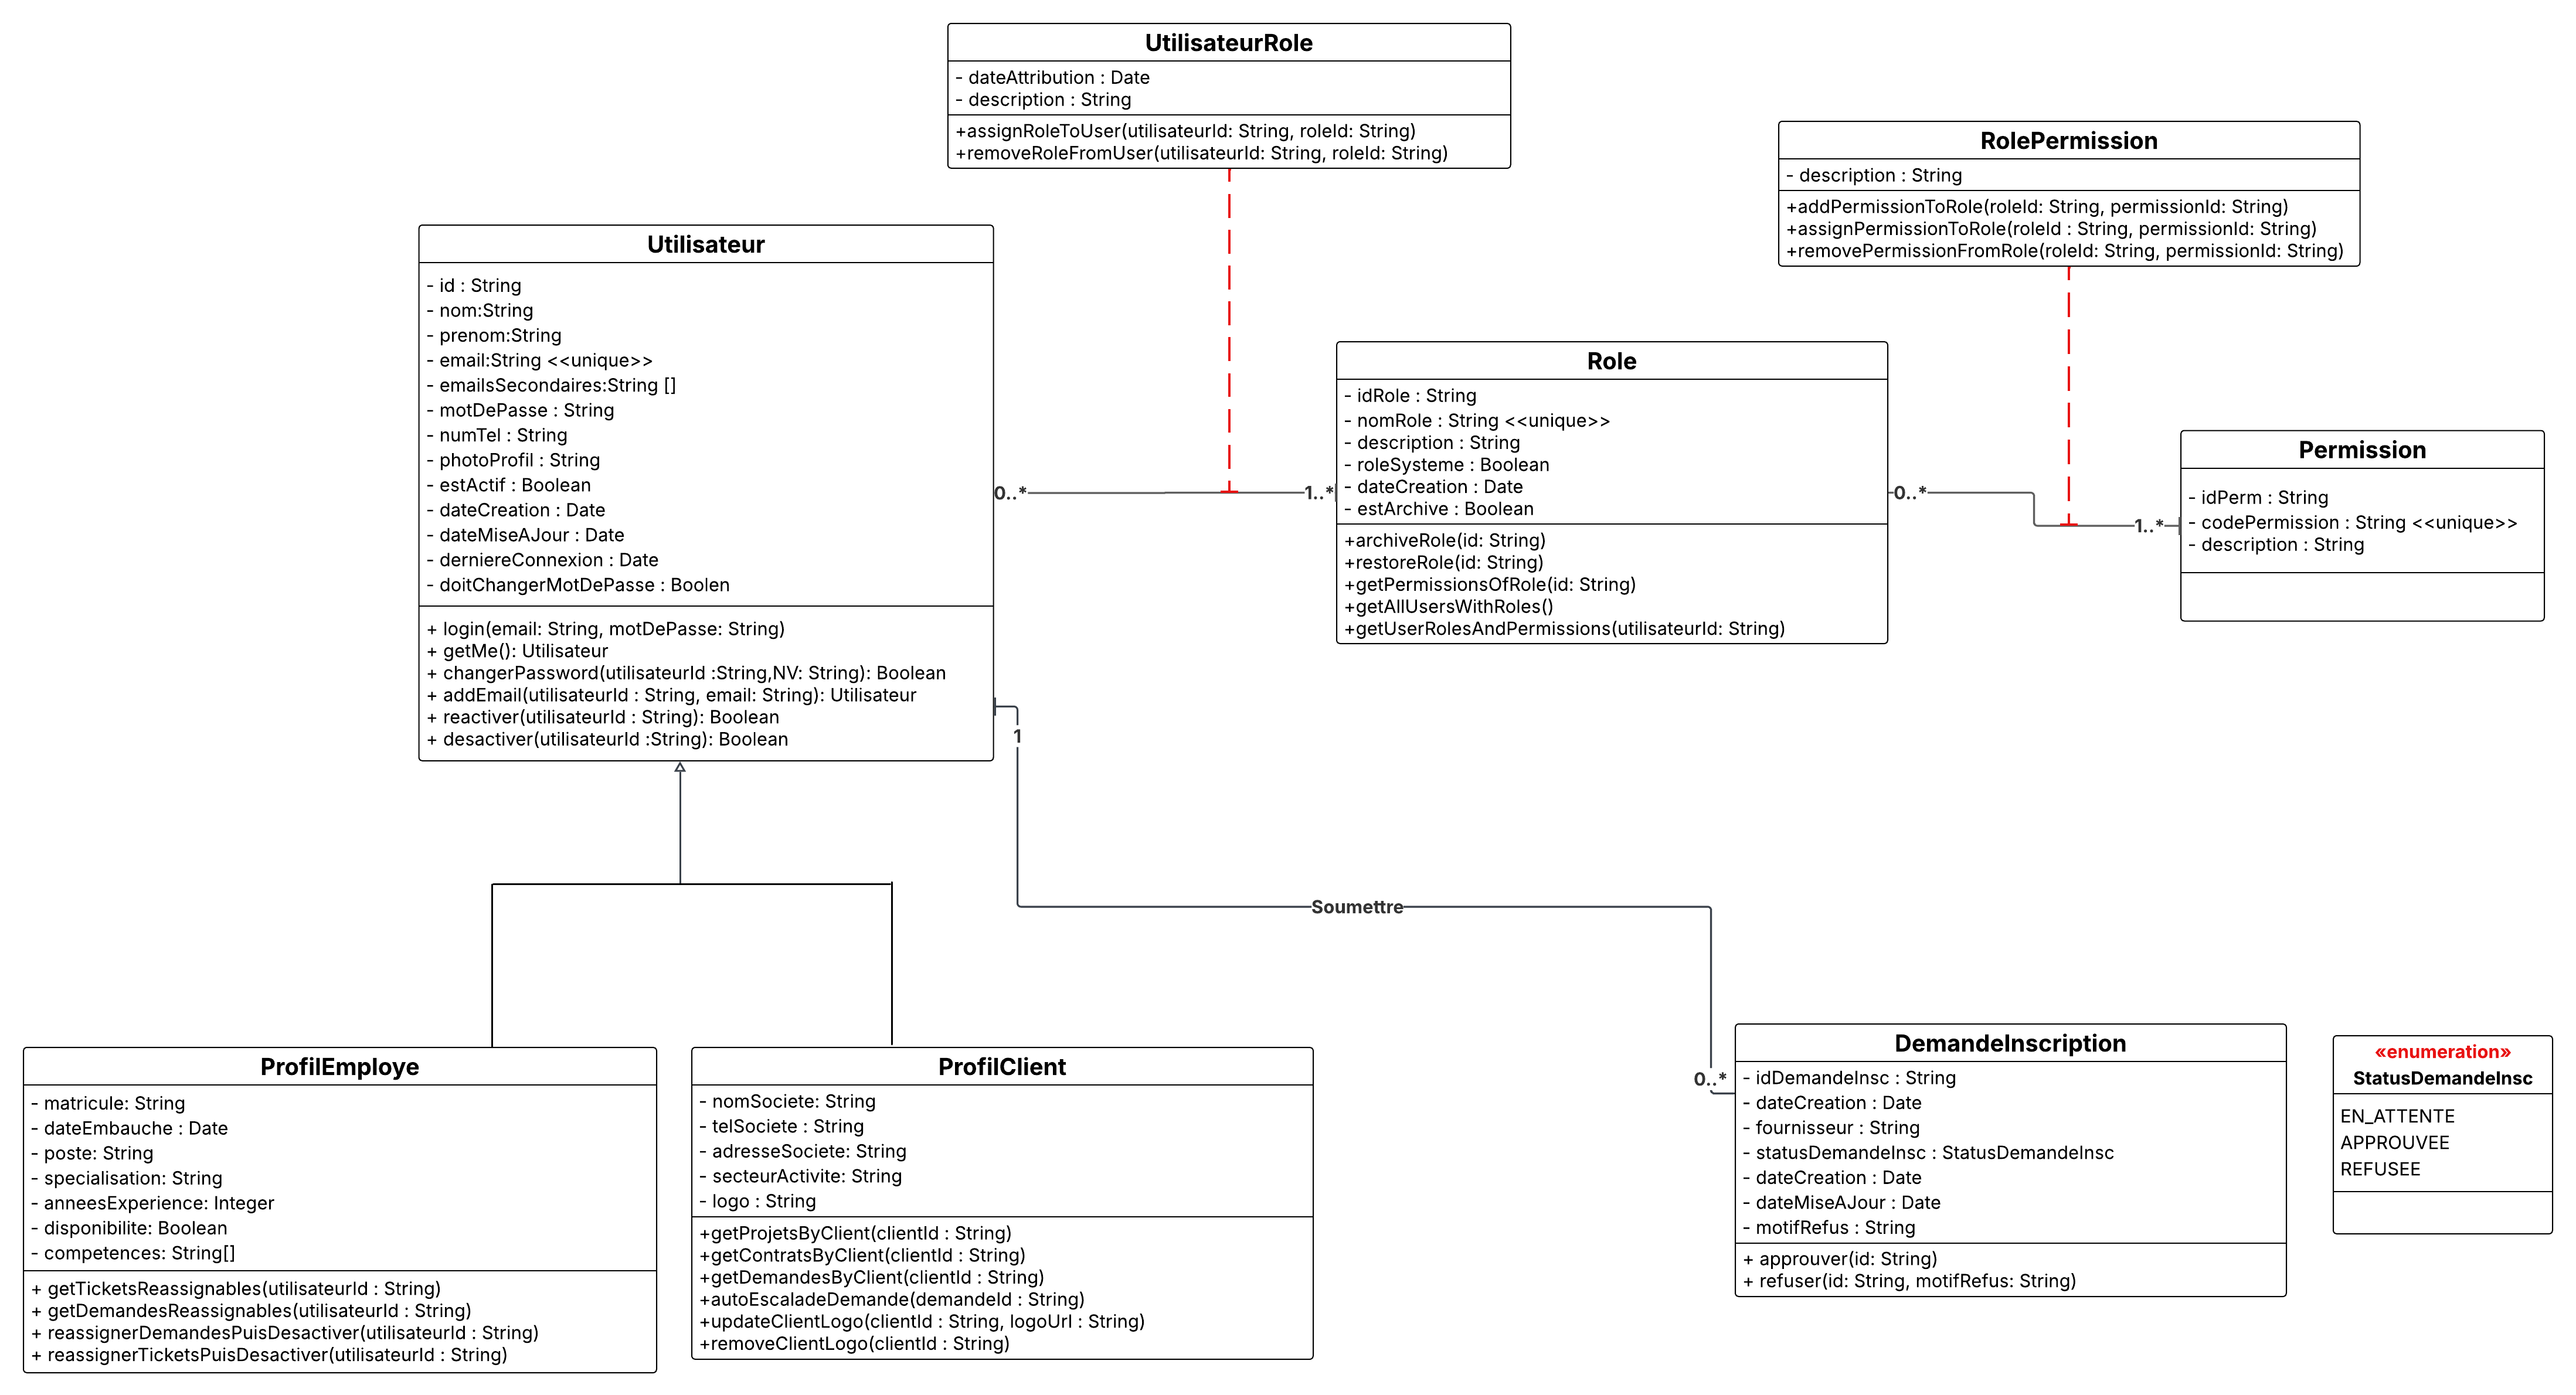
\includegraphics[width=1\textwidth,keepaspectratio]{Images/diag classe sprint 1.png}
        \caption{Diagramme de classes du Sprint 1}
        \label{fig:diag_classe_sprint1}
\end{figure}

\section{Diagramme de séquence}

\subsection{Diagramme de séquences du cas d'utilisation « S'authentifier »}

\begin{figure}[H]
        \centering
        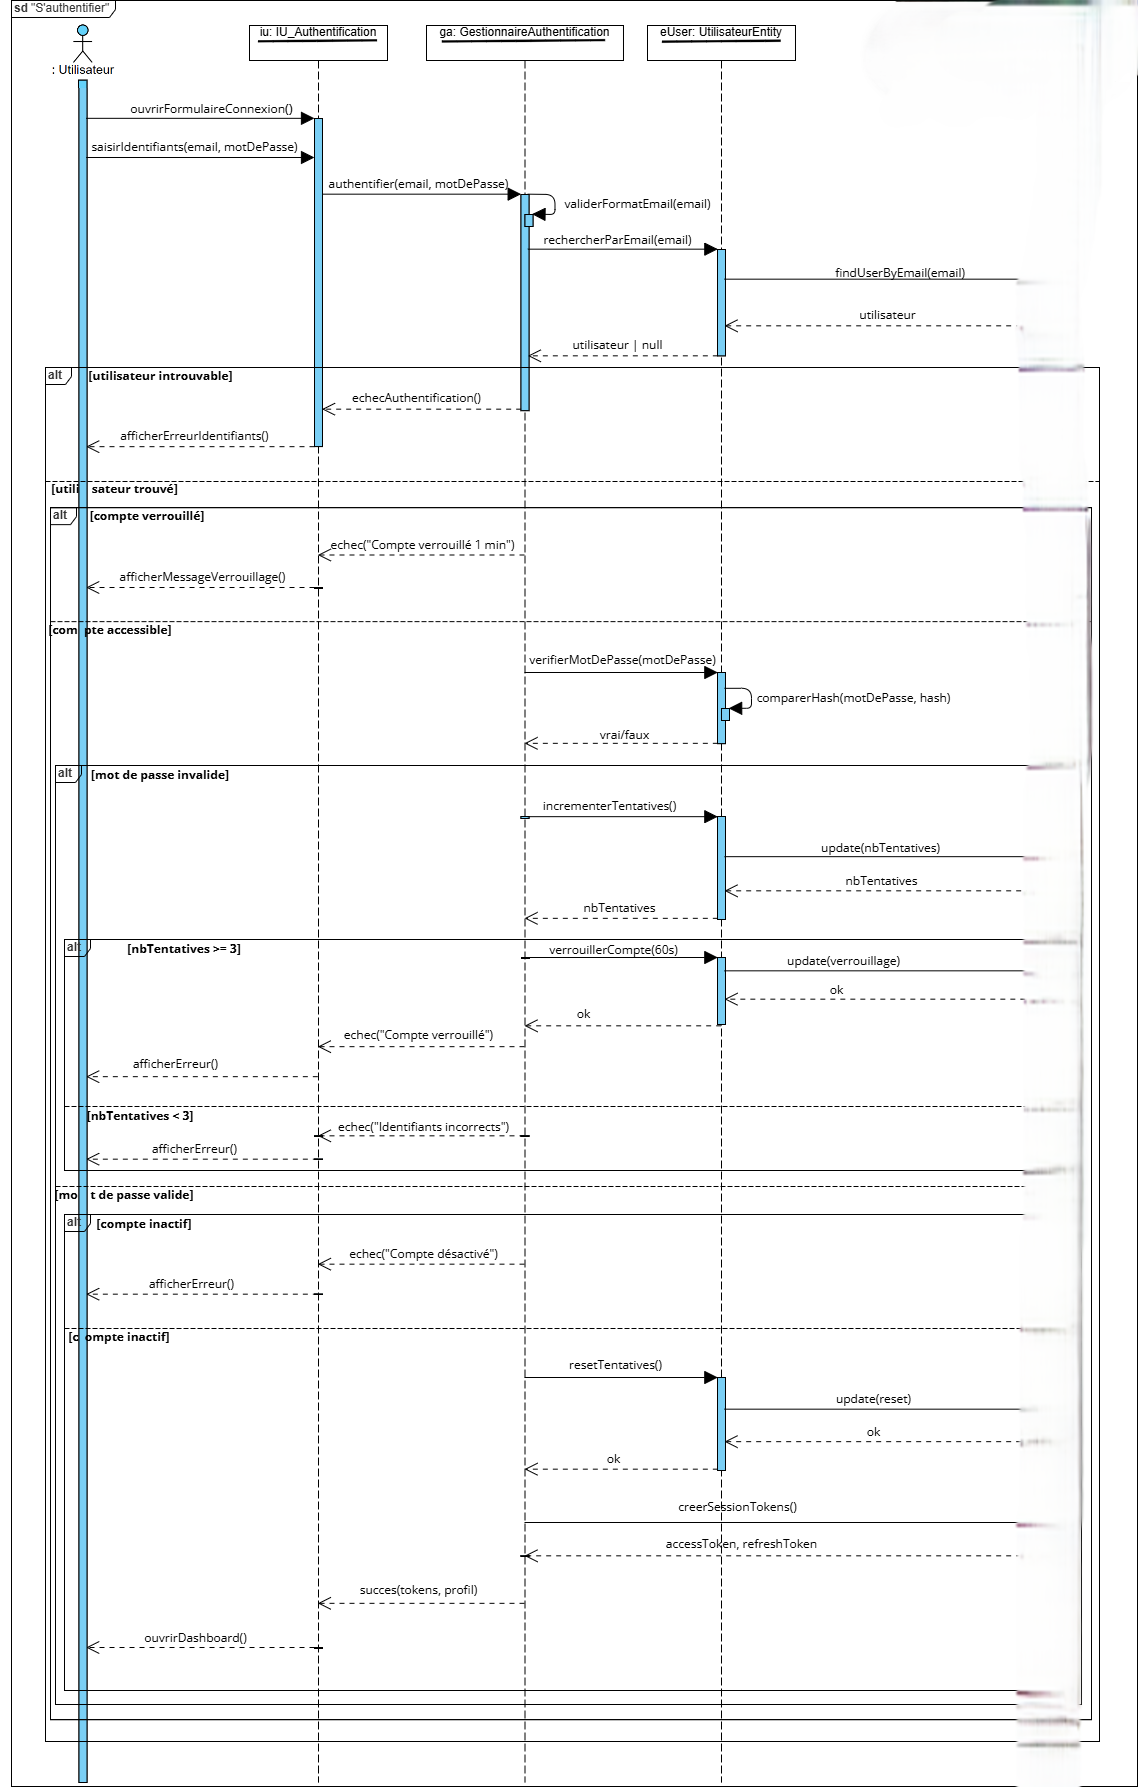
\includegraphics[width=0.7\textwidth,keepaspectratio]{Images/diag_seq_auth.png}
        \caption{Diagramme de séquence du cas d'utilisation « S'authentifier »}
        \label{fig:auth_sequence}
\end{figure}

\subsection{Diagramme de séquences du cas d'utilisation « Mot de passe oublié »}

\begin{figure}[H]
        \centering
        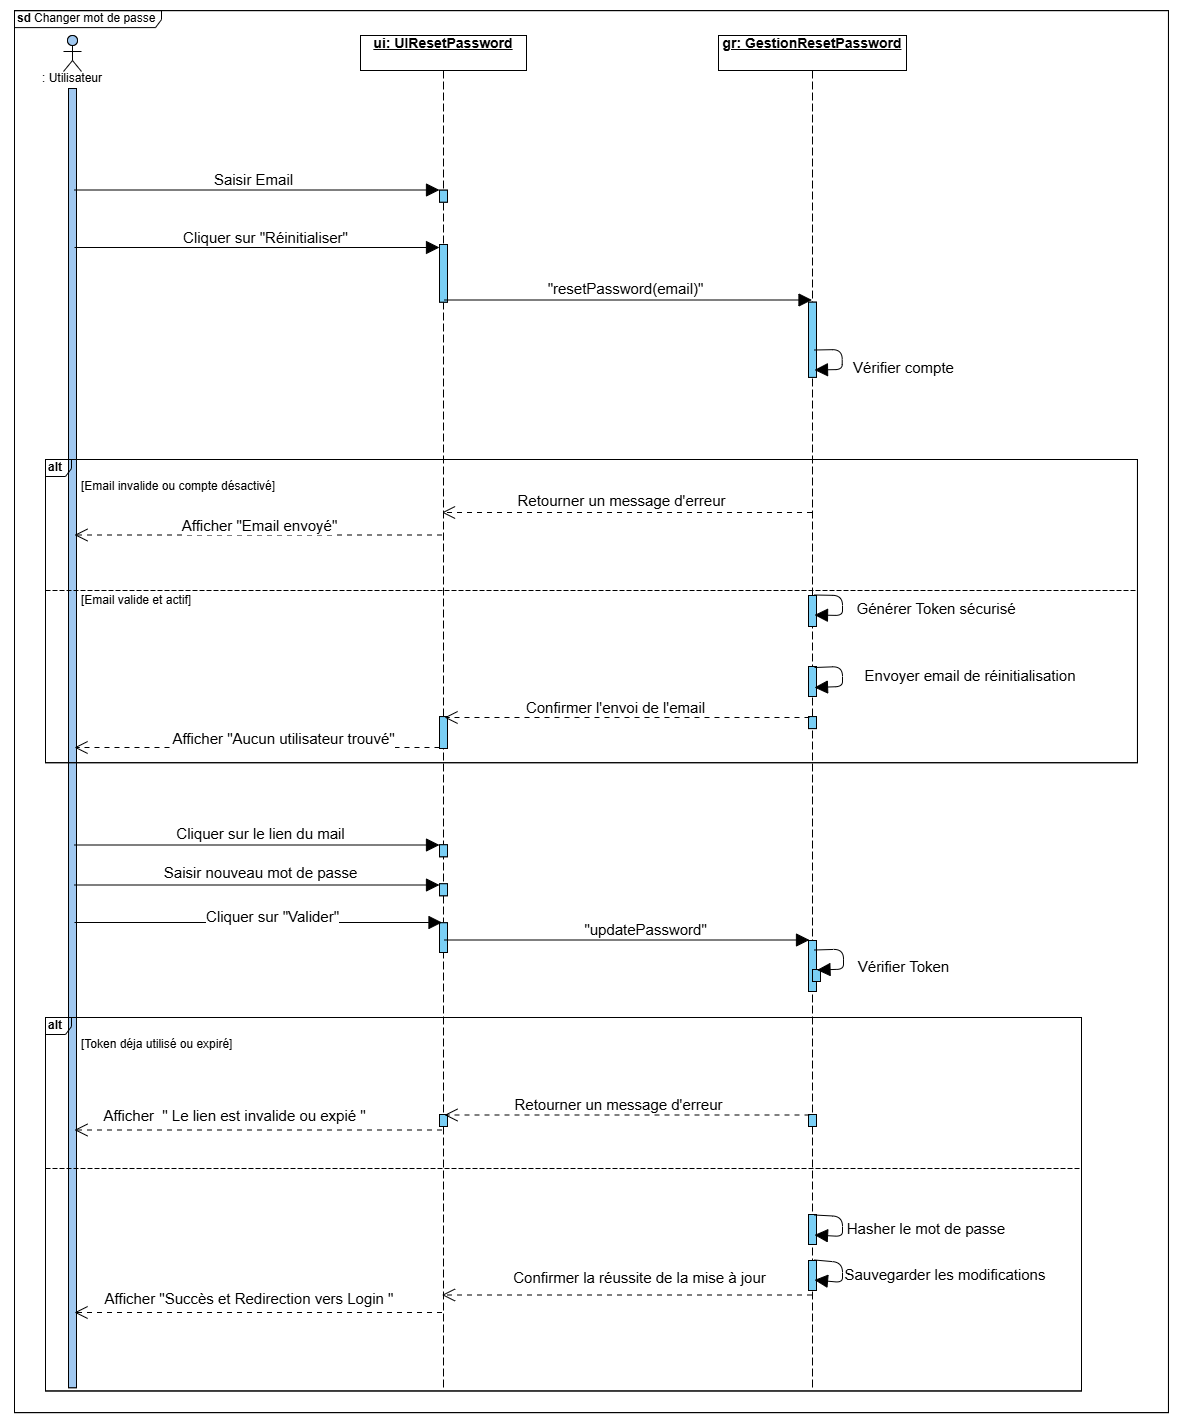
\includegraphics[width=0.7\textwidth,keepaspectratio]{Images/Diagramme changer Mot de passe.png}
        \caption{Diagramme de séquence du cas d'utilisation « Mot de passe oublié »}
        \label{fig:password_reset_sequence}
\end{figure}

\subsection{Diagramme de séquences du cas d'utilisation « Désactiver utilisateur »}

\begin{figure}[H]
        \centering
        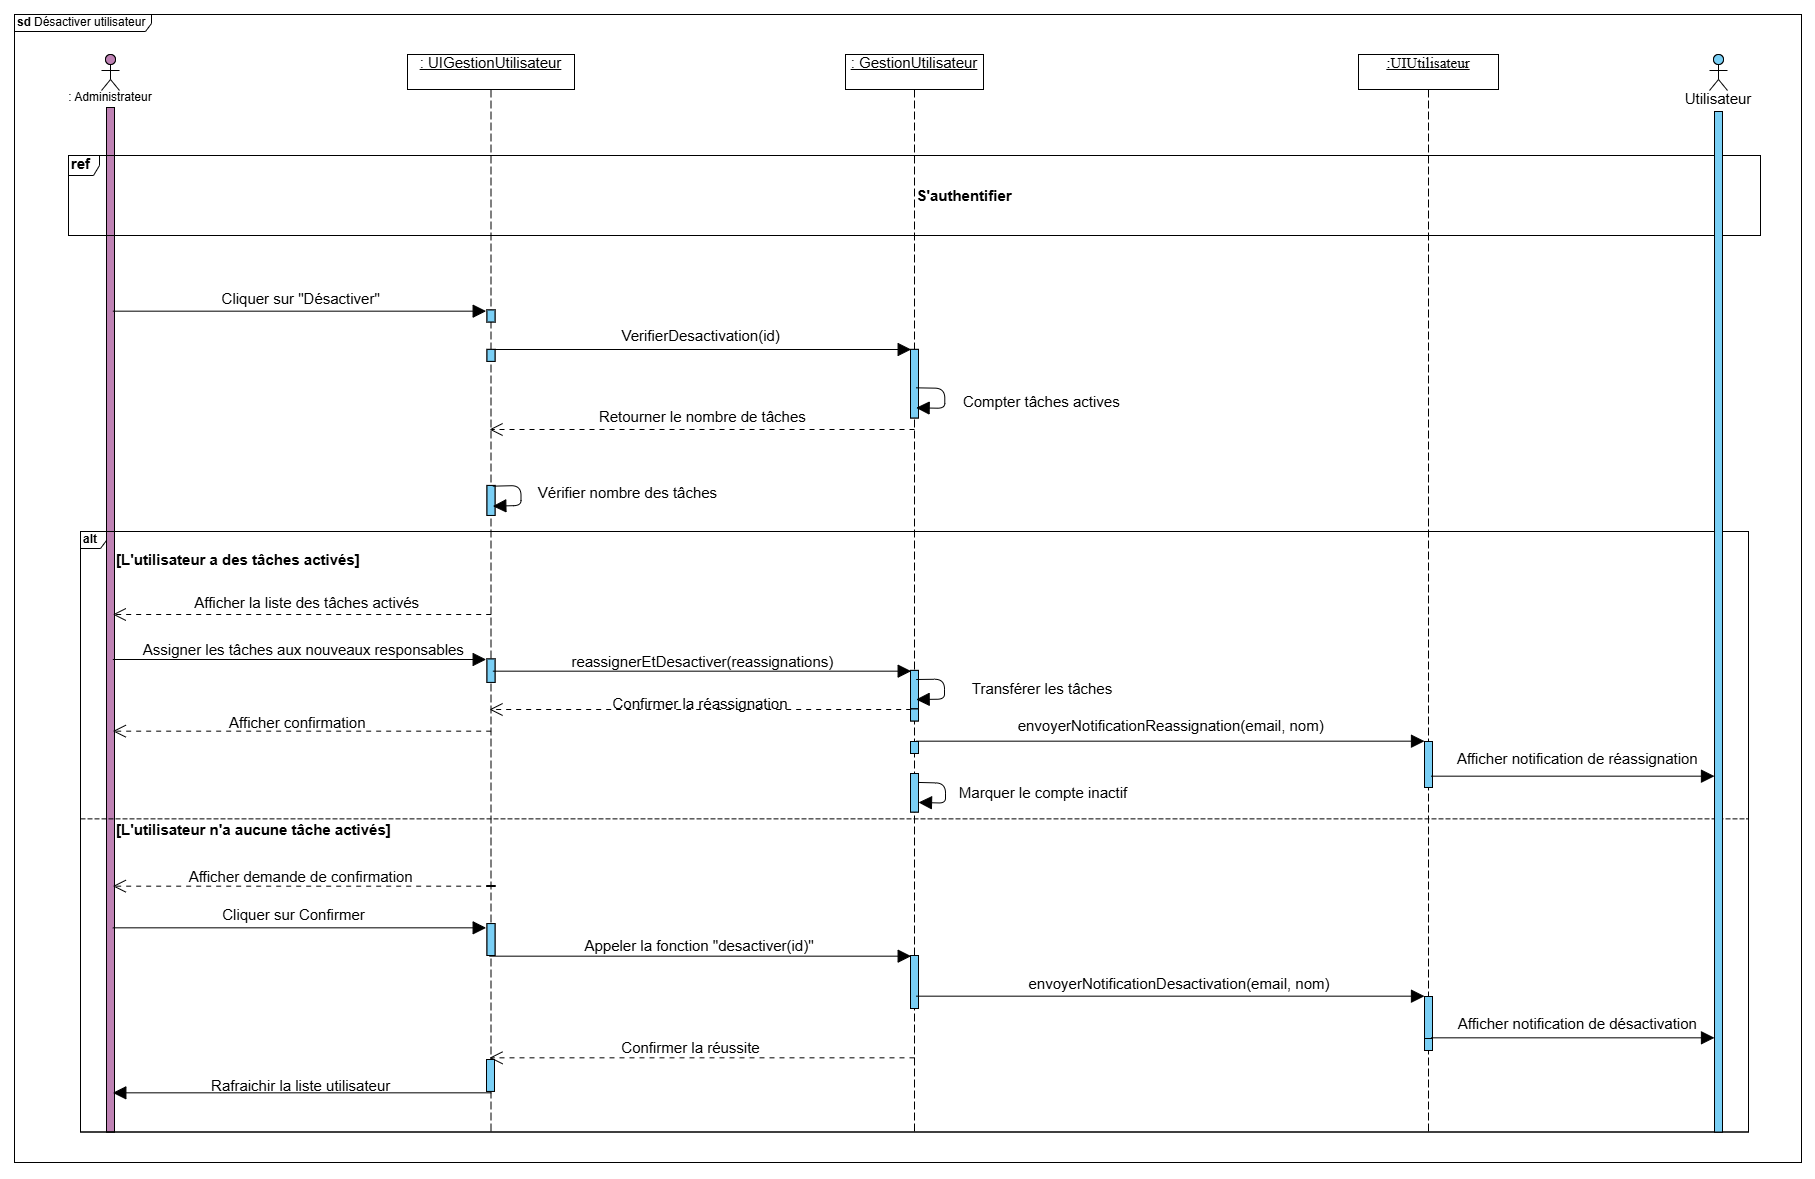
\includegraphics[width=0.7\textwidth,keepaspectratio]{Images/Diaggramme de séquence de Désactiver utilisateur.png}
        \caption{Diagramme de séquence du cas d'utilisation « Désactiver utilisateur »}
        \label{fig:deactivate_user_sequence}
\end{figure}

\subsection{Diagramme d'activité « Authentification et Demander accés via fournisseur externe »}

\begin{figure}[htbp]
        \centering
        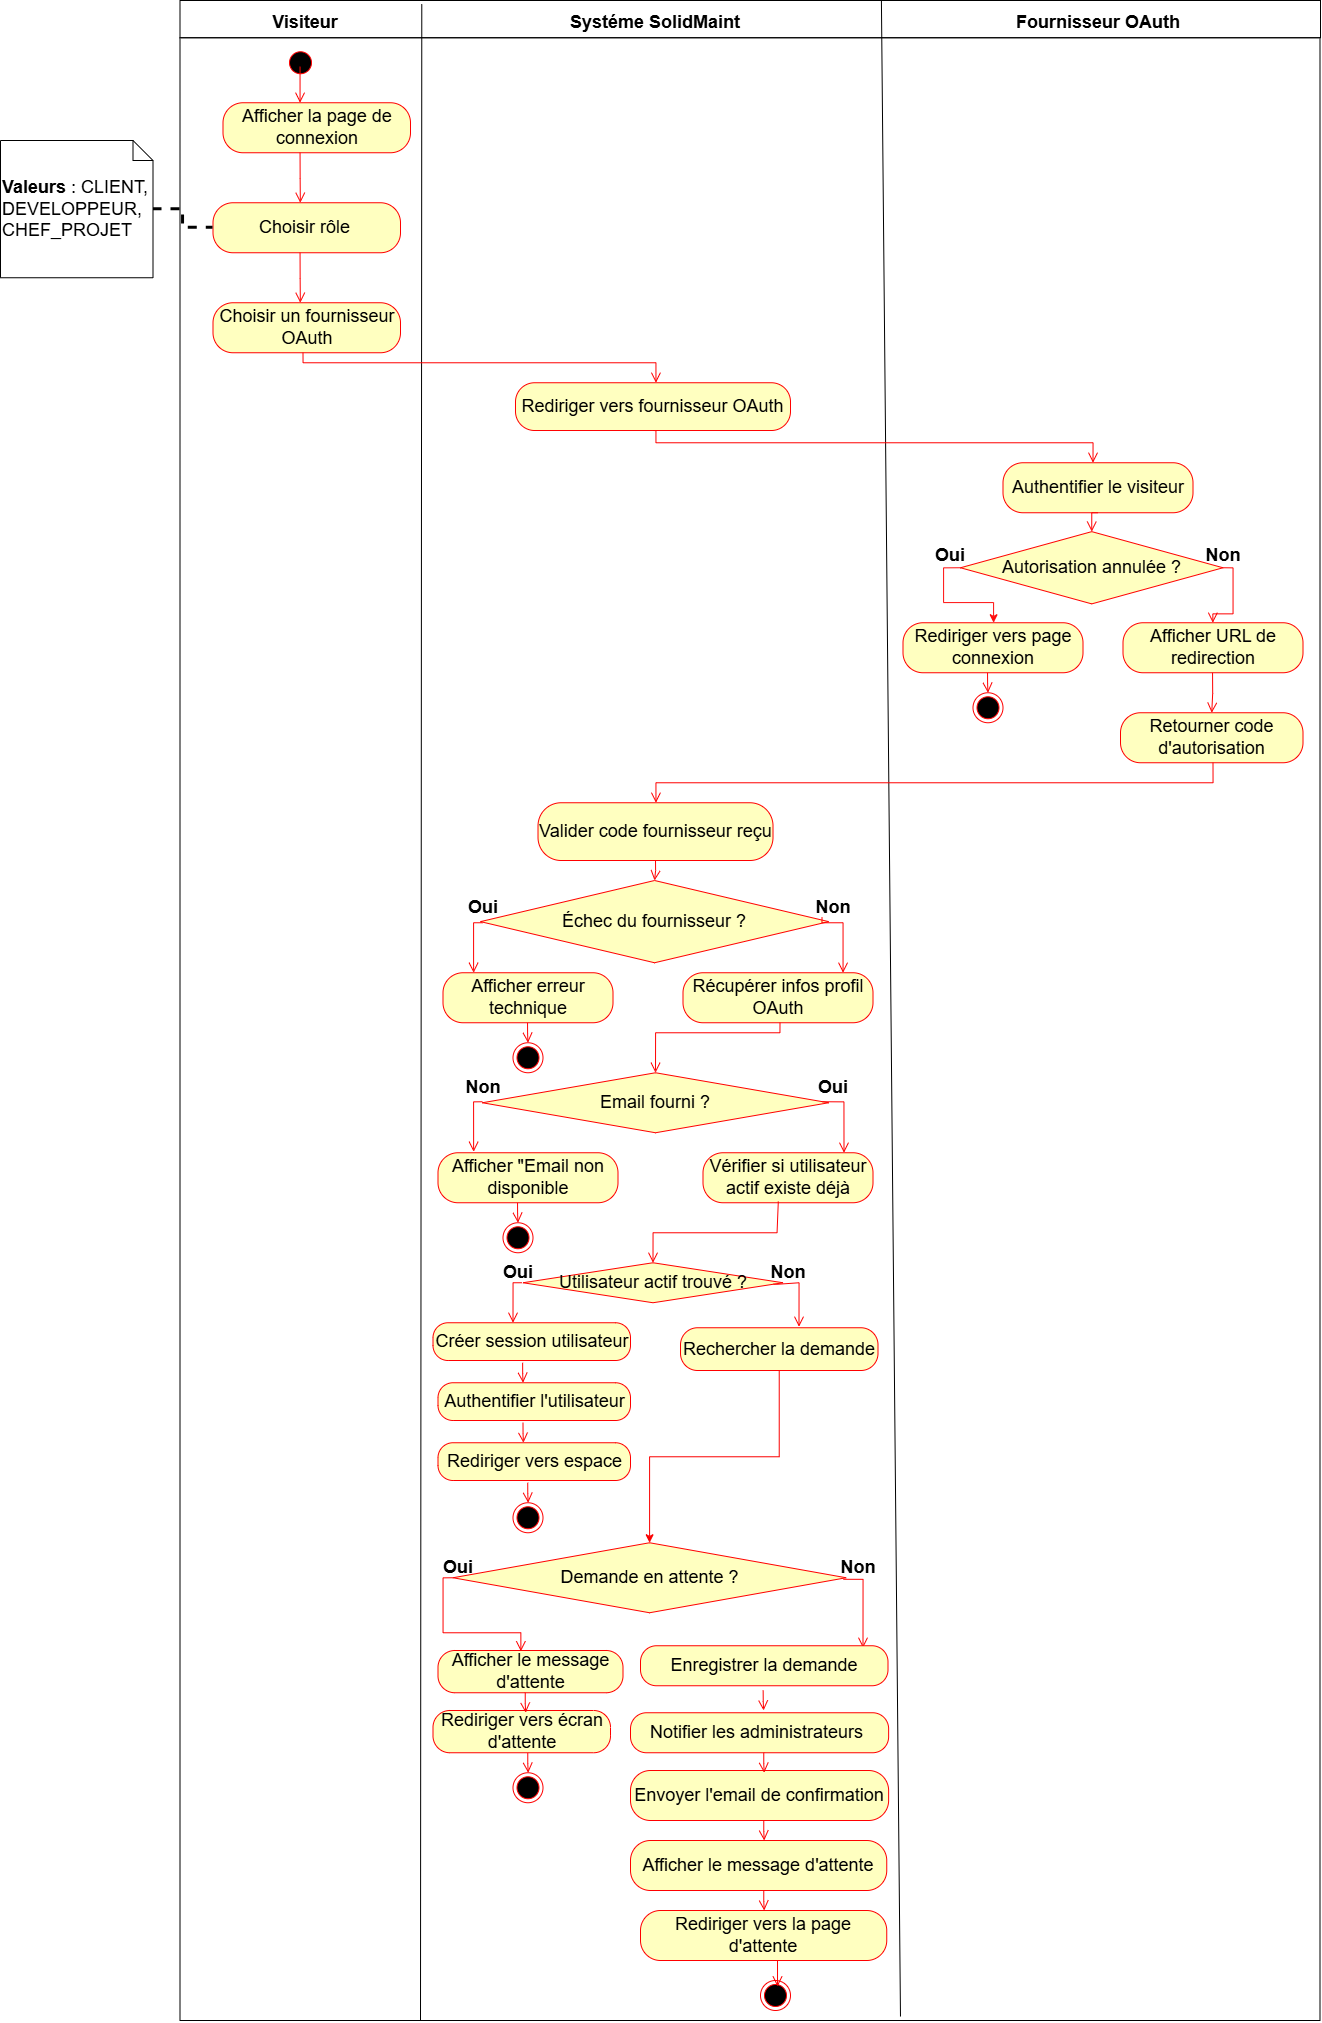
\includegraphics[width=0.9\textwidth,keepaspectratio]{Images/diag_activites_demande_insc.png}
        \caption{Diagramme d'activité d'authentification et Demande accés via fournisseur externe}
        \label{fig:oauth_activity_diagram}
\end{figure}

\section{Schéma relationnel}

\textbf{Utilisateur} (\underline{idUtilisateur}, nom, prenom, email,
  motDePasse, estActif, doitChangerMotDePasse, tentativesConnexionEchouees,
  compteVerrouilleJusquA, photoProfil, dateCreation)
\newline
\textbf{ProfilEmploye} (\underline{idProfilE}, \textbf{\#idUtilisateur},
  matricule, poste, specialisation, disponibilite, dateEmbauche,
  niveauSeniorite)
\newline
\textbf{ProfilClient} (\underline{idProfilC}, \textbf{\#idUtilisateur},
  nomSociete, adresseSociete, secteurActivite, telSociete, logo)
\newline
\textbf{Role} (\underline{idRole}, nomRole, description, roleSysteme,
  estArchive, dateCreation)
\newline
\textbf{Permission} (\underline{idPermission}, codePermission, description)
\newline
\textbf{UtilisateurRole} (\underline{idUtilisateurRole},
  \textbf{\#idUtilisateur}, \textbf{\#idRole}, dateAttribution)
\newline
\textbf{RolePermission} (\underline{idRolePermission}, \textbf{\#idRole},
  \textbf{\#idPermission})
\newline
\textbf{DemandeInscriptionOAuth} (\underline{idDemande}, email, prenom, nom,
  fournisseur, photoProfil, role, statut, dateCreation, motifRefus)
% ─────────────────────────────────────────────────────────────────────────────
% SECTION 4 : RÉALISATION
% ─────────────────────────────────────────────────────────────────────────────

\section{Réalisation}
Après avoir analysé les besoins et conçu les solutions, nous passons maintenant à la réalisation. Dans cette phase, nous avons développé toutes les user stories planifiées dans le sprint backlog. Cette section présente le diagramme de composants qui montre l'architecture de notre application, ainsi que les interfaces utilisateur que nous avons créées pour répondre aux besoins des utilisateurs.
\label{sec:realisation_sprint1}

\subsection{Diagramme de composants}


\subsection{Description des interfaces}
Cette section présente les principales interfaces utilisateur développées lors du premier sprint.

\subsubsection{Interface de connexion}
\begin{figure}[H]
\centering
%\includegraphics[width=0.75\textwidth,keepaspectratio]{Images/interface_connexion.png}
\caption{Interface de connexion — authentification classique et OAuth}
\label{fig:interface_connexion}
\end{figure}
La page de connexion propose deux modes d'authentification : le formulaire
classique (e-mail + mot de passe) et les boutons OAuth (Google, GitHub).
En cas de compte inexistant, le visiteur est redirigé vers un flux de
demande d'inscription.

\subsubsection{Interface de réinitialisation du mot de passe}
\begin{figure}[H]
\centering
%\includegraphics[width=0.75\textwidth,keepaspectratio]{Images/interface_reset_password.png}
\caption{Interface de réinitialisation du mot de passe}
\label{fig:interface_reset}
\end{figure}
Cette interface permet à l'utilisateur de saisir son adresse e-mail pour
recevoir un lien de réinitialisation valable 1 heure.

\subsubsection{Interface de gestion des utilisateurs}
\begin{figure}[H]
\centering
%\includegraphics[width=0.85\textwidth,keepaspectratio]{Images/interface_users.png}
\caption{Interface d'administration — liste des utilisateurs}
\label{fig:interface_users}
\end{figure}
L'administrateur dispose d'une vue en grille ou en liste, avec filtres par
statut et par rôle, barre de recherche et actions rapides (modifier,
désactiver, voir le profil).

\subsubsection{Interface de gestion des rôles et permissions}
\begin{figure}[H]
\centering
%\includegraphics[width=0.85\textwidth,keepaspectratio]{Images/interface_roles_permissions.png}
\caption{Interface d'administration — gestion des rôles et permissions}
\label{fig:interface_roles}
\end{figure}
La matrice des permissions affiche les rôles en colonnes et les catégories
de permissions en lignes, avec des cases à cocher pour une attribution
visuelle et intuitive.

\subsubsection{Interface de gestion des Demandes d'accès via fournisseur externe}
\begin{figure}[H]
\centering
%\includegraphics[width=0.85\textwidth,keepaspectratio]{Images/interface_demandes_oauth.png}
\caption{Interface d'administration — demandes d'inscription OAuth}
\label{fig:interface_oauth}
\end{figure}
L'administrateur consulte les demandes en attente, visualise les
informations récupérées via OAuth et peut approuver ou refuser chaque
demande avec un motif de refus facultatif.

% ─────────────────────────────────────────────────────────────────────────────
% SECTION 5 : TESTS
% ─────────────────────────────────────────────────────────────────────────────
\section{Tests et Validation}
La phase de test est essentielle pour garantir la qualité et la fiabilité de la solution. Elle valide que chaque fonctionnalité répond aux exigences métier et identifie les anomalies avant la mise en production. Dans ce sprint, nous avons testé les mécanismes d'authentification, la gestion des utilisateurs et le contrôle d'accès (RBAC) pour assurer la robustesse de nos implémentations.

\subsection{Stratégie de tests adoptée}
Afin de garantir la qualité et la fiabilité de l'application, nous avons adopté une stratégie de tests structurée, reposant sur une répartition des vérifications à plusieurs niveaux. Cette approche permet d'assurer une bonne couverture fonctionnelle avec un temps d'exécution raisonnable, tout en facilitant l'identification rapide des anomalies.

Les tests ont été organisés par module fonctionnel afin d'assurer une meilleure traçabilité des vérifications effectuées. Ainsi, les tests unitaires couvrent les règles métier les plus fines, les tests d'intégration valident les échanges avec l'API, et les tests End-to-End reproduisent les scénarios complets d'utilisation de l'application.

La pyramide de tests se compose donc de trois niveaux complémentaires :


\subsubsection{Tests unitaires}
\label{sec:tests_unitaires}

Les tests unitaires ont été réalisés à l'aide du framework \textbf{Vitest},
en isolant chaque service du reste de l'application grâce à des mocks
Prisma. Cette approche garantit l'indépendance des tests et permet une
détection précoce des anomalies dès la phase de développement. Trois
modules prioritaires ont été couverts : l'authentification, le contrôle
d'accès basé sur les rôles (RBAC) et la gestion des clients.


\noindent\textbf{Bilan : 45 tests exécutés — 45 réussis — 0 échec.}
\vspace{6pt}

\begin{itemize}[leftmargin=0pt]

% ── 1. Authentification ───────────────────────────────────────────────────────
\item[$\square$] \textbf{Module Authentification}
\newline
\newline
\textit{Méthodes : \texttt{login()} ·
\texttt{demanderReinitialisationMotDePasse()} ·
\texttt{reinitialiserMotDePasse()}}

\noindent Cette suite valide le processus d'authentification classique,
la génération des jetons JWT et le mécanisme de réinitialisation du mot
de passe. Les cas suivants ont été couverts :

\begin{itemize}[label=$\bullet$, nosep, itemsep=2pt]
  \item Un utilisateur actif fournit des identifiants valides : les jetons
    \texttt{accessToken} et \texttt{refreshToken} sont générés
    correctement.
  \item L'adresse e-mail fournie n'existe pas en base de données : la
    connexion est rejetée avec le code \texttt{401 Unauthorized}.
  \item Le mot de passe fourni est incorrect : la connexion est rejetée
    avec le code \texttt{401 Unauthorized}.
  \item L'utilisateur échoue l'authentification \textbf{3 fois
    consécutives} : le compte est verrouillé automatiquement pendant
    \textbf{1 minute} (\texttt{maxLoginAttempts = 3}).
  \item L'utilisateur tente de se connecter alors que son compte est
    verrouillé : la connexion est rejetée avec un message explicite.
  \item Le compte de l'utilisateur est désactivé : la connexion est
    rejetée avec le code \texttt{401 Unauthorized}.
  \item L'adresse e-mail fournie pour la réinitialisation est inexistante :
    une \texttt{NotFoundException} est levée.
  \item Le token de réinitialisation a été généré depuis plus d'une heure :
    une \texttt{BadRequestException} est levée.
\end{itemize}
\begin{figure}[htbp]
\centering
\begin{minipage}{0.48\textwidth}
  \centering
  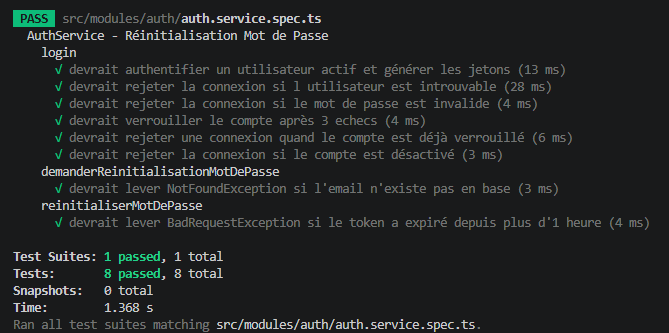
\includegraphics[width=\textwidth,keepaspectratio]
    {Images/test-unitaire-auth.png}
  \caption*{\small Auth}
\end{minipage}
\end{figure}
% ── 2. RBAC ───────────────────────────────────────────────────────────────────
\item[$\square$] \textbf{Module Gestion des rôles et permissions (RBAC)}
\newline
\textit{Méthodes :} \texttt{creerPermission()},
\texttt{attribuerRoleUtilisateur()},
\texttt{obtenirRolesEtPermissions()}
\noindent Cette suite valide les règles d'exclusivité des rôles, l'unicité
des permissions et l'intégrité des références.
\newline
Les cas suivants ont été couverts :

\begin{itemize}[label=$\bullet$, nosep, itemsep=2pt]
  \item Une permission est créée avec un code unique : elle est enregistrée
    correctement en base de données.
  \item Une permission est créée avec un code déjà existant : une
    \texttt{BadRequestException} est levée.
  \item Les rôles et permissions d'un utilisateur sont récupérés : la liste
    est retournée sans doublons.
  \item Un rôle est attribué à un utilisateur sans rôle existant :
    l'attribution est réussie.
  \item L'utilisateur cible est inexistant : une \texttt{NotFoundException}
    est levée.
  \item La règle d'exclusivité \texttt{CLIENT} et \texttt{CHEF\_PROJET}
    est violée : une \texttt{BadRequestException} est levée.
  \item La règle d'exclusivité \texttt{CLIENT} et \texttt{DEVELOPPEUR}
    est violée : une \texttt{BadRequestException} est levée.
  \item La règle d'exclusivité \texttt{CLIENT} et \texttt{ADMIN} est
    violée : une \texttt{BadRequestException} est levée.
  \item La combinaison \texttt{ADMIN} et \texttt{CHEF\_PROJET} est
    soumise : l'attribution est \textbf{autorisée} et réussie.
  \item Le rôle est déjà attribué à l'utilisateur : une
    \texttt{BadRequestException} est levée (doublon détecté).
  \item Le rôle à attribuer est inexistant : une \texttt{NotFoundException}
    est levée.
\end{itemize}
\begin{figure}[htbp]
   \centering
\begin{minipage}{0.48\textwidth}
  \centering
  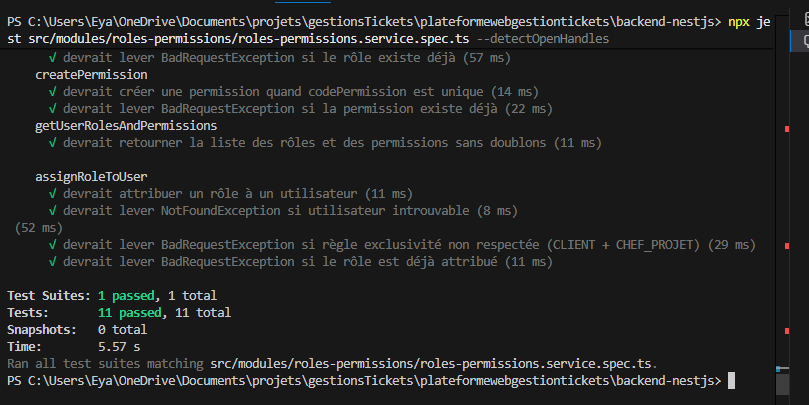
\includegraphics[width=\textwidth,keepaspectratio]{Images/test-sprint1-moduleRole+Permession.png}
  \caption*{\small RBAC}
\end{minipage}
\caption{Résultats des tests unitaires — Auth et RBAC}
\label{fig:test_unitaires}
\end{figure}
% ── 3. Gestion des clients ────────────────────────────────────────────────────

\end{itemize}

\subsubsection{Tests d'intégration}
\label{sec:tests_integration}

Les tests d'intégration ont pour objectif de valider les échanges entre
les différentes couches de l'application (contrôleur, service et base de
données) en testant les endpoints REST dans leur ensemble. Ces tests sont
effectués via \textbf{Swagger UI} en soumettant des requêtes HTTP réelles
contre le backend en cours d'exécution, ce qui permet de vérifier le
comportement de l'API dans des conditions proches de la production.

\begin{itemize}[leftmargin=0pt]

\item[$\square$] \textbf{Authentification}
 \newline
\newline\textit{Endpoint : \texttt{POST /api/auth/login}}

\noindent Cette suite valide le comportement complet de l'endpoint de
connexion, notamment le retour des jetons d'authentification, des rôles,
des permissions associées et la gestion des codes d'erreur HTTP selon les
différents cas d'entrée.
\newline Les cas suivants ont été couverts :

\begin{itemize}[label=$\bullet$, nosep, itemsep=2pt]
  \item Un utilisateur actif de rôle \texttt{ADMIN} fournit des
    identifiants valides : l'endpoint retourne le code \textbf{200 OK}
    accompagné des champs \texttt{accessToken}, \texttt{refreshToken},
    des données de l'utilisateur, de ses rôles et de la liste complète
    de ses permissions.
  \item L'adresse e-mail fournie n'existe pas en base de données :
    l'endpoint retourne le code \textbf{401 Unauthorized}.
  \item Le mot de passe fourni est incorrect : l'endpoint retourne le
    code \textbf{401 Unauthorized}.
  \item Les données soumises sont invalides (adresse e-mail mal formatée
    ou champ obligatoire vide) : l'endpoint retourne le code
    \textbf{400 Bad Request} accompagné d'un message de validation
    généré par \texttt{class-validator}.
  \item Le compte de l'utilisateur est désactivé
    (\texttt{estActif = false}) : l'endpoint retourne le code
    \textbf{401 Unauthorized} avec le message
    « Ce compte est désactivé ».
\end{itemize}

\begin{figure}[H]
\centering
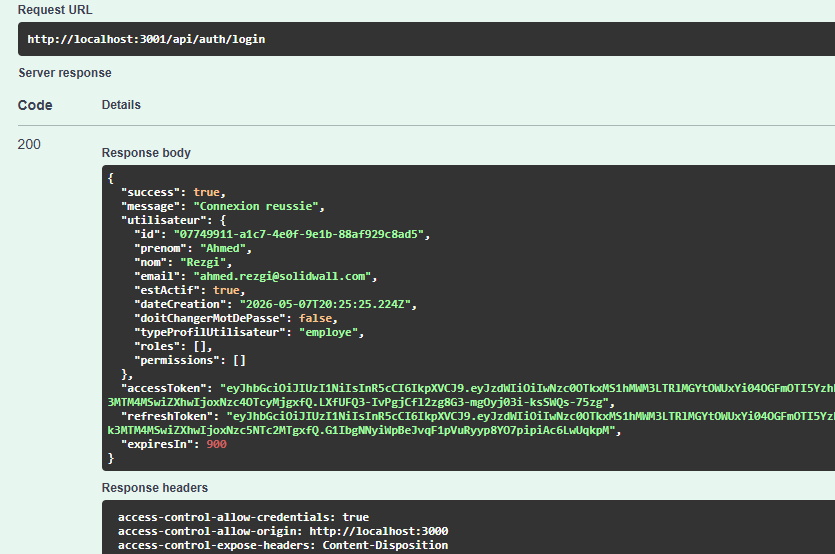
\includegraphics[width=0.60\textwidth,keepaspectratio]
  {Images/test-interg-login.png}
\caption{Test d'intégration — endpoint \texttt{POST /api/auth/login}
  via Swagger}
\label{fig:test_integration}
\end{figure}

\item[$\square$]  \textbf {Gestion du profil}
\newline
\newline\textit{Endpoint : \texttt{PUT /api/profil}}
 
\noindent Cette suite de tests vise à valider le bon fonctionnement de la méthode \textbf{modifierProfil()} exposée via l'endpoint \textbf{PUT /api/profil}, qui permet à un utilisateur de mettre à jour les informations de son profil.
\newline
Lee cas suivant ont été couvert :
\begin{itemize}
\item[$\bullet$] Cas où l'e-mail fourni dans la requête ne respecte pas le format attendu.
\end{itemize}
\begin{figure}[htbp]
        \centering
        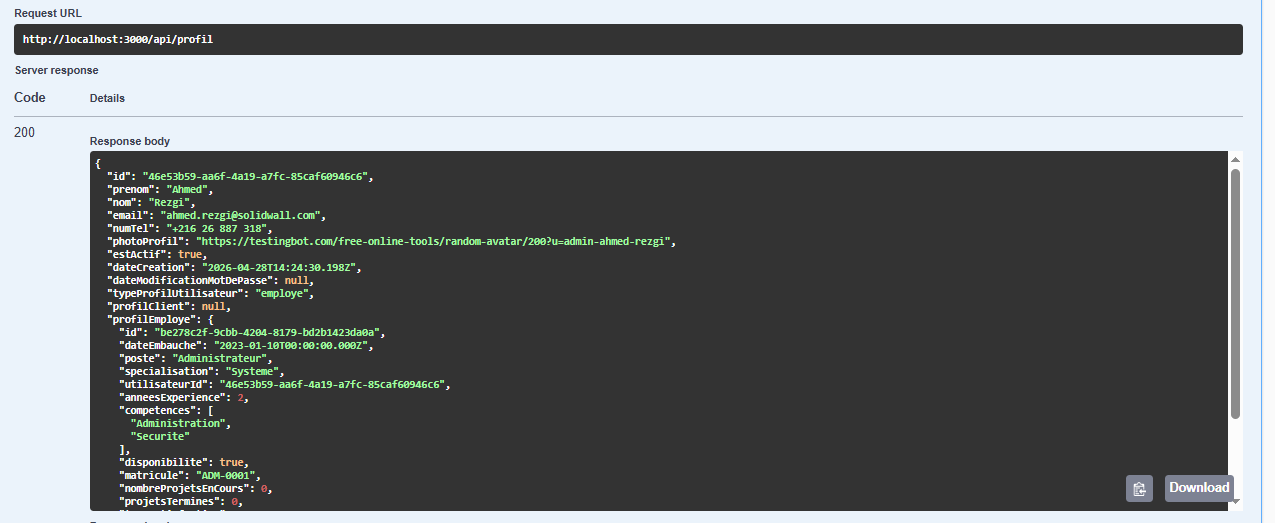
\includegraphics[width=0.7\textwidth,keepaspectratio]{Images/gestion profil Swagger.png}
        \caption{Test de mise à jour du profil}
    \end{figure}
\end{itemize}

\subsubsection{Tests End-to-End}
\label{sec:tests_e2e}

Les tests End-to-End ont pour objectif de simuler les parcours utilisateurs
complets dans un navigateur réel piloté par \textbf{Playwright}. Ces tests
s'exécutent en interaction avec le frontend Next.js, le backend NestJS et
la base de données PostgreSQL, reproduisant ainsi les conditions réelles
d'utilisation de la plateforme.
\newline

\noindent\textbf{Bilan : 11 tests exécutés — 11 réussis — 0 échec.}
\vspace{6pt}

\begin{itemize}[leftmargin=0pt]

\item[$\square$] \textbf{Authentification}
\newline
\newline\textit{10 scénarios : connexion classique, OAuth, déconnexion}

\noindent Cette suite valide le flux complet d'authentification en
simulant les actions réelles d'un utilisateur sur l'interface. Les cas
suivants ont été couverts :

\begin{itemize}[label=$\bullet$, nosep, itemsep=2pt]
  \item La page de connexion est chargée : le formulaire et les boutons
    d'authentification OAuth sont affichés correctement.
  \item Les champs du formulaire sont vides ou partiellement remplis :
    le bouton de soumission reste désactivé.
  \item L'utilisateur soumet des identifiants valides : le flux aboutit
    à une redirection vers la page d'accueil et une session est créée.
  \item L'utilisateur saisit un identifiant ou un mot de passe invalide :
    un message d'erreur approprié est affiché sans redirection.
  \item L'utilisateur échoue l'authentification \textbf{3 fois
    consécutives} : le compte est verrouillé pendant \textbf{1 minute}
    et un message d'information est affiché.
  \item L'utilisateur se déconnecte : les jetons sont supprimés du
    \texttt{localStorage} et l'utilisateur est redirigé vers la page
    \texttt{/connexion}.
  \item L'utilisateur s'authentifie via \textbf{Google} avec succès :
    les données du profil sont récupérées et une session valide est
    créée.
  \item L'authentification via \textbf{Google} échoue : un message
    d'erreur technique est affiché.
  \item L'utilisateur s'authentifie via \textbf{GitHub} avec succès :
    les données du profil sont récupérées et une session valide est
    créée.
  \item L'authentification via \textbf{GitHub} échoue : un message
    d'erreur technique est affiché.
\end{itemize}

\begin{figure}[H]
\centering
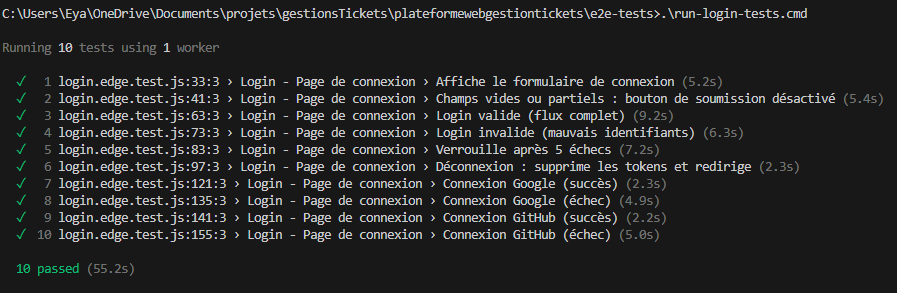
\includegraphics[width=0.68\textwidth,keepaspectratio]
  {Images/ExecDeTestCasesReussi-auth.png}
\caption{Tests End-to-End — Authentification via Playwright}
\label{fig:test_e2e_auth}
\end{figure}

\item[$\square$] \textbf{Gestion des utilisateurs} ---
\textit{1 scénario : désactivation avec réassignation des tickets}

\noindent Cette suite valide le flux complet de désactivation d'un
utilisateur disposant de tickets actifs, en simulant les actions réelles
d'un administrateur. Le cas suivant a été couvert :

\begin{itemize}[label=$\bullet$, nosep, itemsep=2pt]
  \item L'administrateur tente de désactiver un utilisateur actif
    disposant de \textbf{9 tickets actifs} (statuts \texttt{OUVERT},
    \texttt{EN\_COURS} ou \texttt{EN\_REVUE}) : le système affiche le
    modal de réassignation présentant la liste des développeurs
    disponibles \textbf{triés par charge de travail croissante}.
    L'administrateur procède à la réassignation de chaque ticket, puis
    confirme l'opération via le bouton « Réassigner et Désactiver ».
    Le système effectue les réassignations dans une transaction atomique,
    désactive le compte et envoie un e-mail de notification à
    l'utilisateur concerné.
\end{itemize}

\begin{figure}[H]
\centering
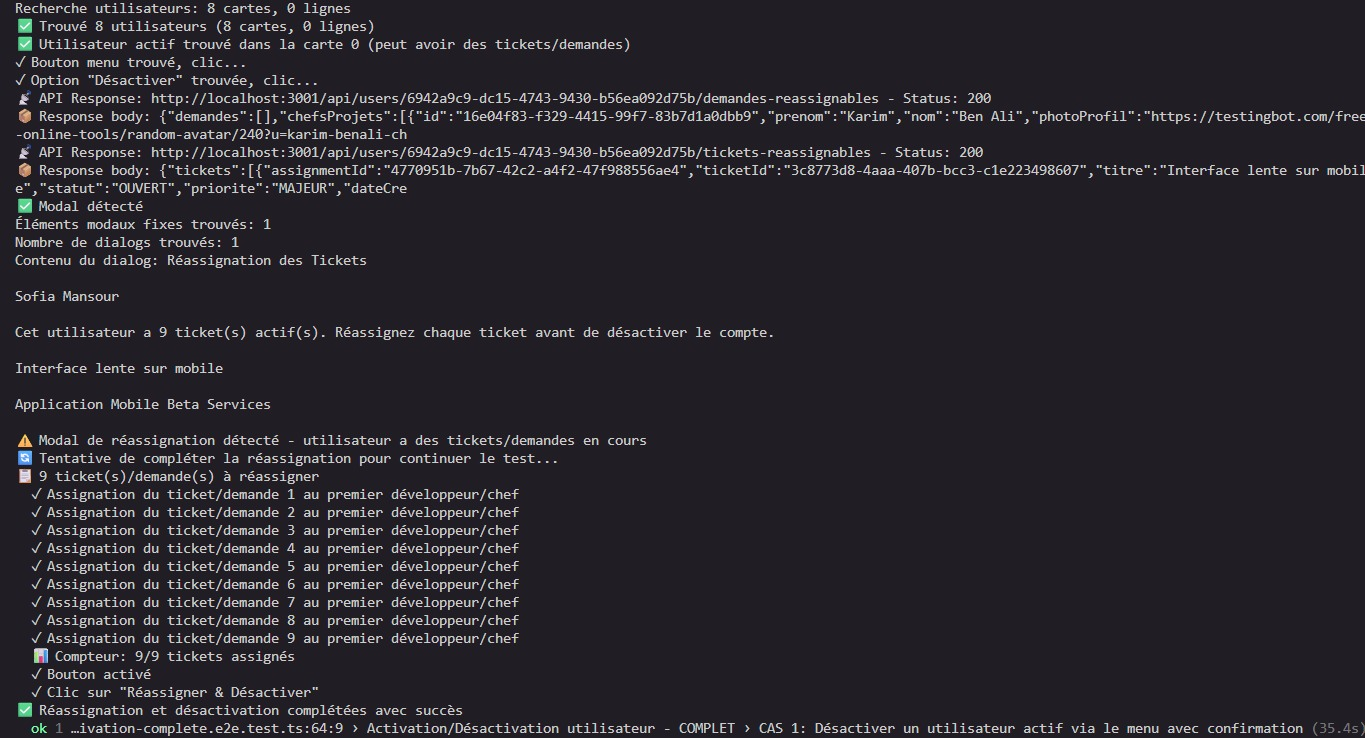
\includegraphics[width=0.68\textwidth,keepaspectratio]
  {Images/Test e2e desactiver utilisateu.png}
\caption{Tests End-to-End — Désactivation utilisateur via Playwright}
\label{fig:test_e2e_desactiver}
\end{figure}

\end{itemize}